\documentclass[a4paper]{article}

\def\npart {IA}
\def\nterm {Michaelmas}
\def\nyear {2014}
\def\nlecturer {M.\ G.\ Worster}
\def\ncourse {Differential Equations}

\input{header}

\begin{document}
\maketitle
{\small
  \noindent\textbf{Basic calculus}\\
  Informal treatment of differentiation as a limit, the chain rule, Leibnitz's rule, Taylor series, informal treatment of $O$ and $o$ notation and l'H\^opital's rule; integration as an area, fundamental theorem of calculus, integration by substitution and parts.\hspace*{\fill}[3]

  \vspace{5pt}
  \noindent Informal treatment of partial derivatives, geometrical interpretation, statement (only) of symmetry of mixed partial derivatives, chain rule, implicit differentiation. Informal treatment of differentials, including exact differentials. Differentiation of an integral with respect to a parameter.\hspace*{\fill}[2]

  \vspace{10pt}
  \noindent\textbf{First-order linear differential equations}\\
  Equations with constant coefficients: exponential growth, comparison with discrete equations, series solution; modelling examples including radioactive decay.

  \vspace{5pt}
  \noindent Equations with non-constant coefficients: solution by integrating factor.\hspace*{\fill}[2]

  \vspace{10pt}
  \noindent\textbf{Nonlinear first-order equations}\\
  Separable equations. Exact equations. Sketching solution trajectories. Equilibrium solutions, stability by perturbation; examples, including logistic equation and chemical kinetics. Discrete equations: equilibrium solutions, stability; examples including the logistic map.\hspace*{\fill}[4]

  \vspace{10pt}
  \noindent\textbf{Higher-order linear differential equations}\\
  Complementary function and particular integral, linear independence, Wronskian (for second-order equations), Abel's theorem. Equations with constant coefficients and examples including radioactive sequences, comparison in simple cases with difference equations, reduction of order, resonance, transients, damping. Homogeneous equations. Response to step and impulse function inputs; introduction to the notions of the Heaviside step-function and the Dirac delta-function. Series solutions including statement only of the need for the logarithmic solution.\hspace*{\fill}[8]

  \vspace{10pt}
  \noindent\textbf{Multivariate functions: applications}\\
  Directional derivatives and the gradient vector. Statement of Taylor series for functions on $\R^n$. Local extrema of real functions, classification using the Hessian matrix. Coupled first order systems: equivalence to single higher order equations; solution by matrix methods. Non-degenerate phase portraits local to equilibrium points; stability.

  \vspace{5pt}
  \noindent Simple examples of first- and second-order partial differential equations, solution of the wave equation in the form $f(x + ct) + g(x - ct)$.\hspace*{\fill}[5]}
\tableofcontents

\setcounter{section}{-1}
\section{Introduction}
In this course, it is assumed that students already know how to do calculus. While we will define all of calculus from scratch, it is there mostly to introduce the big and small $o$ notation which will be used extensively in this and future courses (as well as for the sake of completeness). It is impossible for a person who hasn't seen calculus before to learn calculus from those few pages.

Calculus is often used to model physical systems. For example, if we know that the force $F = m\ddot x$ on a particle at any time $t$ is given by $t^2 - 1$, then we can write this as
\[
  m\ddot x = t^2 - 1.
\]
We can easily integrate this twice with respect to $t$, and find the position $x$ as a function of time.

However, often the rules governing a physical system are not like this. Instead, the force on the particle is more likely to depend on the \emph{position} of the particle, instead of what time it is. Hence the actual equation of motion might be
\[
  m\ddot x = x^2 - 1.
\]
This is an example of a \emph{differential equation}. We are given an equation that a function $x$ obeys, often involving derivatives of $x$, and we have to find all functions that satisfy this equation (of course, the first equation is also a differential equation, but a rather boring one).

A closely related notion is \emph{difference equations}. These are discrete analogues of differential equations. A famous example is the \emph{Fibonacci sequence}, which states that
\[
  F_{n + 2} - F_{n + 1} - F_n = 0.
\]
This specifies a relationship between terms in a sequence $(F_n)$, and we want to find an explicit solution to this equation.

In this course, we will develop numerous techniques to solve different differential equations and difference equations. Often, this involves guessing of some sort.

\section{Differentiation}
This section provides a brief review of differentiation, with particular emphasis on the asymptotic notation that will be used throughout this course.

\subsection{Definition of the derivative}
\begin{defi}[Derivative of function]
  Let $f$ be a real-valued function defined on an open interval containing the point $x$. The \emph{derivative} of $f$ with respect to $x$, interpreted as the rate of change of $f(x)$ with $x$, is
  \[
    \frac{\d f}{\d x} = \lim_{h\to 0} \frac{f(x + h) - f(x)}{h},
  \]
  provided this limit exists. The function $f$ is said to be \emph{differentiable} at $x$ if this limit exists (equivalently, if the left-hand and right-hand limits are equal).
\end{defi}

\begin{eg}[Absolute value at origin]
  Consider the absolute value function $f(x)=|x|$. This function is not differentiable at $x = 0$, since the left-hand and right-hand limits differ: $\lim\limits_{h\to 0^+} \frac{|h| - |0|}{h}= 1$ while $\lim\limits_{h\to 0^-} \frac{|h| - |0|}{h}= -1$.
\end{eg}

\begin{notation}
  Several notations are commonly used for derivatives. We write
  \[
    \frac{\d f}{\d x} = f'(x) = \frac{\d}{\d x} f(x).
  \]
  Higher derivatives are denoted similarly: $\frac{\d}{\d x}\left(\frac{\d f}{\d x}\right) = \frac{\d^2 f}{\d x^2} = f''(x)$.

  The prime notation $f'$ always denotes the derivative with respect to the function's argument. For example, if $g(t) = f(2t)$, then $g'(t) = 2f'(2t)$ by the chain rule.
\end{notation}

\subsection{Small \texorpdfstring{$o$}{o} and big \texorpdfstring{$O$}{O} notations}
\begin{defi}[$O$ and $o$ notations]
  Let $f$ and $g$ be real-valued functions, and let $x_0$ be a point (possibly $\pm\infty$).
  \begin{enumerate}
    \item We write ``$f(x) = o(g(x))$ as $x\to x_0$'' if $\lim\limits_{x\to x_0} \frac{f(x)}{g(x)} = 0$. Intuitively, this means $f(x)$ is much smaller than $g(x)$ near $x_0$.
    \item We write ``$f(x) = O(g(x))$ as $x\to x_0$'' if $\frac{f(x)}{g(x)}$ remains bounded as $x\to x_0$. Intuitively, this means $f(x)$ is at most comparable in size to $g(x)$ near $x_0$.

      Note that for $f(x) = O(g(x))$ to hold, the limit $\displaystyle \lim_{x\to x_0} \frac{f(x)}{g(x)}$ need not exist.
  \end{enumerate}
  In practice, $x_0$ is typically either $0$ or $\infty$. Observe that $f(x)=o(g(x))$ implies $f(x) = O(g(x))$.
\end{defi}
\begin{remark}
  The notation $f(x) = o(g(x))$ is an abuse of notation. The symbol $o(g(x))$ does not denote a specific function; rather, it represents a \emph{class} of functions (namely, all functions satisfying the property above). The statement ``$f(x) = o(g(x))$'' means that $f$ belongs to this class. A more precise notation would be $f(x) \in o(g(x))$, but the equality notation is standard and more convenient in practice.
\end{remark}

\begin{eg}[Big-O and little-o examples]\leavevmode
  \begin{itemize}
    \item $x=o(\sqrt{x})$ as $x\to 0$, since $\frac{x}{\sqrt{x}} = \sqrt{x} \to 0$. Conversely, $\sqrt{x} = o(x)$ as $x\to \infty$.
    \item $\sin 2x = O(x)$ as $x\to 0$, since $\sin 2x \approx 2x$ for small $x$.
    \item $\sin 2x = O(1)$ as $x\to \infty$, even though $\lim_{x\to\infty} \sin 2x$ does not exist. Here, the ratio $\frac{\sin 2x}{1}$ remains bounded (between $-1$ and $1$).
  \end{itemize}
\end{eg}

This notation is used frequently in analysis. For example, to express that all terms of order two or higher in $h$ are being neglected, one writes $+O(h^2)$. The notation provides an alternative characterization of the derivative.
\begin{prop}[Linear approximation characterization]
  Let $f$ be a differentiable function and let $x_0$ be a point in its domain. Then as $h \to 0$,
  \[
    f(x_0 + h) = f(x_0) + f'(x_0)h + o(h).
  \]
\end{prop}

\begin{proof}
  By the definition of the derivative,
  \[
    f'(x_0) = \lim_{h\to 0}\frac{f(x_0 + h) - f(x_0)}{h}.
  \]
  This means $\frac{f(x_0 + h) - f(x_0)}{h} - f'(x_0) \to 0$ as $h \to 0$, which can be written as
  \[
    f(x_0 + h) - f(x_0) - f'(x_0)h = o(h).
  \]
  Rearranging gives the result.
\end{proof}

\subsection{Methods of differentiation}
\begin{thm}[Chain rule]
  Let $g$ be a function differentiable at $x$, and let $F$ be a function differentiable at $g(x)$. If $f$ is defined by the composition $f(x) = F(g(x))$, then
  \[
    \frac{\d f}{\d x} = \frac{\d F}{\d g}\frac{\d g}{\d x}.
  \]
\end{thm}

\begin{proof}
  Since $g$ is differentiable at $x$, by the linear approximation characterization we have $g(x + h) = g(x) + hg'(x) + o(h)$ as $h \to 0$. Similarly, since $F$ is differentiable at $g(x)$, for any increment $k$ we have $F(g(x) + k) = F(g(x)) + kF'(g(x)) + o(k)$ as $k \to 0$. Setting $k = hg'(x) + o(h)$, which tends to $0$ as $h \to 0$, we obtain
  \begin{align*}
    \frac{\d f}{\d x} &= \lim_{h\to 0}\frac{F(g(x + h)) - F(g(x))}{h}\\
    &= \lim_{h\to 0}\frac{F(g(x) + hg'(x) + o(h)) - F(g(x))}{h}\\
    &= \lim_{h\to 0}\frac{(hg'(x) + o(h))F'(g(x)) + o(hg'(x) + o(h))}{h}\\
    &= \lim_{h\to 0}\left(g'(x)F'(g(x)) + \frac{o(h)}{h}\right)\\
    &= g'(x)F'(g(x)) = \frac{\d F}{\d g}\frac{\d g}{\d x}.\qedhere
  \end{align*}
\end{proof}

\begin{thm}[Product Rule]
  Let $u$ and $v$ be differentiable functions of $x$, and define $f(x) = u(x)v(x)$. Then
  \[
    f'(x) = u'(x)v(x) + u(x)v'(x).
  \]
\end{thm}

\begin{proof}
  Using the linear approximation characterization, we have $u(x+h) = u(x) + hu'(x) + o(h)$ and similarly for $v$. Then
  \begin{align*}
    f(x+h) &= u(x+h)v(x+h) \\
    &= (u(x) + hu'(x) + o(h))(v(x) + hv'(x) + o(h)) \\
    &= u(x)v(x) + h(u'(x)v(x) + u(x)v'(x)) + o(h).
  \end{align*}
  The result follows from the linear approximation characterization applied to $f$.
\end{proof}

\begin{thm}[Leibniz's Rule]
  Let $u$ and $v$ be $n$-times differentiable functions of $x$, where $n$ is a non-negative integer, and let $f = uv$. Then the $n$-th derivative of $f$ is given by
  \[
    f^{(n)}(x) = \sum_{r = 0}^n \binom{n}{r}u^{(r)}(x)\,v^{(n - r)}(x),
  \]
  where $u^{(r)}$ denotes the $r$-th derivative of $u$ (with $u^{(0)} = u$), and $\binom{n}{r} = \frac{n!}{r!(n-r)!}$ is the binomial coefficient.
\end{thm}

\begin{proof}
  The proof proceeds by induction on $n$. The base case $n=1$ is the product rule. For the inductive step, differentiate both sides of the formula for $f^{(n)}$ and apply the product rule to each term, using the identity $\binom{n}{r} + \binom{n}{r-1} = \binom{n+1}{r}$.
\end{proof}

\subsection{Taylor's theorem}
Taylor's theorem generalizes the linear approximation characterization to higher orders, expressing a function as a polynomial plus an error term.

\begin{thm}[Taylor's Theorem]
  Let $n$ be a non-negative integer, and let $f$ be a function that is $n$-times differentiable at a point $x$. Then as $h \to 0$,
  \[
    f(x + h) = f(x) + hf'(x) + \frac{h^2}{2!}f''(x) + \cdots + \frac{h^n}{n!}f^{(n)}(x) + E_n,
  \]
  where the error term $E_n$ satisfies $E_n = o(h^{n})$. If additionally $f^{(n+1)}$ exists, then $E_n = O(h^{n+1})$.
\end{thm}

\begin{remark}
  Taylor's Theorem provides only a \emph{local} approximation of $f$ near $x$; it does not, in general, provide information about the behaviour of $f$ far from $x$.

  An equivalent formulation is obtained by substituting $x - x_0$ for $h$, where $x_0$ is a fixed point and $x$ varies:
  \[
    f(x) = f(x_0) + (x-x_0)f'(x_0) + \frac{(x-x_0)^2}{2!}f''(x_0) + \cdots + \frac{(x-x_0)^n}{n!}f^{(n)}(x_0) + E_n.
  \]
\end{remark}

\begin{defi}[Taylor series]
  Let $f$ be an infinitely differentiable function at a point $x_0$. The \emph{Taylor series} of $f$ about $x_0$ is the formal power series
  \[
    \sum_{n=0}^{\infty} \frac{(x-x_0)^n}{n!}f^{(n)}(x_0) = f(x_0) + (x-x_0)f'(x_0) + \frac{(x-x_0)^2}{2!}f''(x_0) + \cdots,
  \]
  obtained by taking the formal limit $n \to \infty$ in Taylor's Theorem.
\end{defi}

\subsection{L'H\^opital's rule}
L'H\^opital's rule provides a method for evaluating limits of indeterminate forms.

\begin{thm}[L'H\^opital's Rule]
  Let $f$ and $g$ be functions that are differentiable at $x_0$, with $f(x_0) = g(x_0) = 0$. If $g'(x_0) \neq 0$, then
  \[
    \lim_{x\to x_0} \frac{f(x)}{g(x)} = \frac{f'(x_0)}{g'(x_0)}.
  \]
  More generally, if $\displaystyle\lim_{x\to x_0} \frac{f'(x)}{g'(x)}$ exists, then $\displaystyle\lim_{x\to x_0} \frac{f(x)}{g(x)} = \lim_{x\to x_0} \frac{f'(x)}{g'(x)}$.
\end{thm}

\begin{proof}
  Since $f$ and $g$ are differentiable at $x_0$, they are continuous there, so the hypothesis $\lim_{x\to x_0}f(x) = \lim_{x\to x_0}g(x) = 0$ implies $f(x_0) = g(x_0) = 0$. By Taylor's Theorem,
  \[
    f(x) = f(x_0) + (x - x_0)f'(x_0) + o(x - x_0) = (x - x_0)f'(x_0) + o(x - x_0),
  \]
  and similarly $g(x) = (x - x_0)g'(x_0) + o(x - x_0)$. Thus
  \begin{align*}
    \lim_{x\to x_0} \frac{f(x)}{g(x)} &= \lim_{x\to x_0} \frac{(x - x_0)f'(x_0) + o(x - x_0)}{(x - x_0)g'(x_0) + o(x - x_0)}\\
    &= \lim_{x\to x_0} \frac{f'(x_0) + \frac{o(x-x_0)}{x-x_0}}{g'(x_0) + \frac{o(x-x_0)}{x-x_0}} = \frac{f'(x_0)}{g'(x_0)}.\qedhere
  \end{align*}
\end{proof}

\section{Integration}
This section introduces integration as the inverse operation to differentiation and presents several techniques for evaluating integrals.

\subsection{Definition of the integral}
\begin{defi}[Integral]
  Let $f$ be a function defined on an interval $[a, b]$. To define the integral of $f$ over $[a, b]$, we partition the interval into $N$ subintervals of equal width $\Delta x = \frac{b-a}{N}$, with endpoints $x_n = a + n\Delta x$ for $n = 0, 1, \ldots, N$. The \emph{integral} of $f$ over $[a, b]$ is defined as the limit of the Riemann sum:
  \[
    \int_a^b f(x) \;\d x = \lim_{N\to\infty}\sum_{n=0}^{N-1} f(x_n)\Delta x.
  \]
  More generally, the term ``integral'' refers to any limit of such sums (the precise definition of the Riemann integral is treated in Analysis I). Pictorially, this represents the area under the curve:
  \begin{center}
    \begin{tikzpicture}
      \draw [->] (-1, 0) -- (5, 0) node [right] {$x$};
      \draw [->] (0, -0.5) -- (0, 5) node [above] {$y$};

      \draw [domain=-1:5] plot (\x, {(\x + 1)*(\x + 1)/10 + 1});

      \draw (0.5, 0) node [below] {$a$} -- (0.5, 1.225) -- (1, 1.225);
      \draw (1, 0) node [below] {$x_1$} -- (1, 1.4) -- (1.5, 1.4);
      \draw (1.5, 0) node [below] {$x_2$} -- (1.5, 1.625) -- (2, 1.625) -- (2, 0) node [below] {$x_3$};
      \node at (2.4, 0.8) {$\cdots$};
      \draw (2.75, 0) node [below] {$x_n$} -- (2.75, 2.40625) -- (3.25, 2.40625) -- (3.25, 0) node [anchor = north west] {$\!\!\!\!\!x_{n + 1}\cdots$};
      \node at (3.65, 1.2) {$\cdots$};
      \draw (4, 0) -- (4, 3.5) -- (4.5, 3.5) -- (4.5, 0) node [below] {$b$};
    \end{tikzpicture}
  \end{center}
\end{defi}

\begin{remark}
  Each rectangle in the Riemann sum has width $\Delta x$ and height $f(x_n)$. For a differentiable function $f$, the true area under the curve over $[x_n, x_{n+1}]$ differs from $f(x_n)\Delta x$ by $O(\Delta x^2)$, since $f$ varies by at most $O(\Delta x)$ over the subinterval. Summing over all $N$ rectangles, the total error is $N \cdot O(\Delta x^2) = O(\Delta x)$ (since $N\Delta x = b - a$ is constant), which vanishes as $N \to \infty$.
\end{remark}

The fundamental connection between differentiation and integration is given by the following theorem.

\begin{thm}[Fundamental Theorem of Calculus]
  Let $f$ be a continuous function on $[a, b]$, and define $F(x) = \int_a^x f(t)\;\d t$ for $x \in [a,b]$. Then $F$ is differentiable and $F'(x) = f(x)$.
\end{thm}

\begin{proof}
  By the definition of the derivative,
  \begin{align*}
    F'(x) &= \lim_{h\to 0}\frac{F(x+h) - F(x)}{h} = \lim_{h\to 0}\frac{1}{h}\left[\int_a^{x+h}f(t)\;\d t - \int_a^x f(t)\;\d t\right]\\
    &= \lim_{h\to 0} \frac{1}{h}\int_x^{x+h}f(t) \;\d t.
  \end{align*}
  Since $f$ is continuous, for small $h$ we have $f(t) = f(x) + O(h)$ for $t \in [x, x+h]$. Thus
  \[
    \int_x^{x+h}f(t)\;\d t = f(x) \cdot h + O(h^2),
  \]
  and dividing by $h$ and taking the limit gives $F'(x) = f(x)$.
\end{proof}
\begin{cor}[Derivatives of integrals with variable limits]
  Let $f$ be a continuous function.
  \begin{enumerate}
    \item If $b$ is a constant, then
    \[
      \frac{\d}{\d x}\int_x^b f(t)\;\d t = -f(x),
    \]
    since $\int_x^b f(t)\,\d t = -\int_b^x f(t)\,\d t$.
    \item More generally, if $g$ is a differentiable function and $a$ is a constant, then by the chain rule,
    \[
      \frac{\d}{\d x}\int_a^{g(x)} f(t)\;\d t = f(g(x))g'(x).
    \]
  \end{enumerate}
\end{cor}

\begin{notation}
  The \emph{indefinite integral} $\int f(x)\;\d x$ denotes an antiderivative of $f$, i.e., any function $F$ such that $F'(x) = f(x)$. Since antiderivatives differ by a constant, we write $\int f(x)\,\d x = F(x) + C$, where $C$ is the \emph{constant of integration}.
\end{notation}

\subsection{Methods of integration}
Integration is substantially harder than differentiation. While the product rule and chain rule, combined with a table of standard derivatives, suffice to differentiate most expressions, many seemingly simple integrands can be surprisingly difficult---or even impossible---to integrate in closed form. This subsection presents several techniques for evaluating integrals.

\subsubsection*{Substitution}
The method of substitution is the integration analogue of the chain rule.

\begin{prop}[Integration by substitution]
  Let $g$ be a differentiable function, and let $f$ be a function such that $f(g(x))$ is integrable. Setting $u = g(x)$, we have
  \[
    \int f(g(x))g'(x)\,\d x = \int f(u)\,\d u.
  \]
\end{prop}

In practice, we write $\d u = g'(x)\,\d x$ and substitute directly.

\begin{eg}[Integration by substitution]
  Consider $\int \frac{1 - 2x}{\sqrt{x - x^2}}\;\d x$. Let $u = x - x^2$, so that $\d u = (1 - 2x)\;\d x$. The integral becomes
  \[
    \int \frac{\d u}{\sqrt{u}} = \int u^{-1/2}\,\d u = 2u^{1/2} + C = 2\sqrt{x - x^2} + C.
  \]
\end{eg}

\subsubsection*{Trigonometric and hyperbolic substitution}
When the integrand contains expressions involving square roots of quadratics, a trigonometric or hyperbolic substitution can simplify the integral. The following table summarizes common substitutions:
\begin{center}
  \begin{tabular}{ccc}
    \toprule
    Useful identity & Part of integrand & Substitution \\
    \midrule
    $\cos^2\theta + \sin^2\theta = 1$ & $\sqrt{1 - x^2}$ & $x = \sin \theta$ \\
    $1 + \tan^2\theta = \sec^2\theta$ & $1 + x^2$ & $x = \tan\theta$ \\
    $\cosh^2u - \sinh^2 u = 1$ & $\sqrt{x^2 - 1}$ & $x=\cosh u$ \\
    $\cosh^2u - \sinh^2 u = 1$ & $\sqrt{1 + x^2}$ & $x=\sinh u$ \\
    $1 - \tanh^2 u = \sech^2u$ & $1 - x^2$ & $x = \tanh u$ \\
    \bottomrule
  \end{tabular}
\end{center}
\begin{eg}[Shifted sine substitution]
  Consider $\int \sqrt{2x - x^2}\;\d x$. Completing the square gives $2x - x^2 = 1 - (x-1)^2$, so we substitute $x - 1 = \sin\theta$, whence $\d x = \cos\theta\,\d\theta$ and $\sqrt{1 - (x-1)^2} = \cos\theta$. The integral becomes
  \begin{align*}
    \int \cos^2\theta \;\d \theta &= \int\frac{1 + \cos 2\theta}{2}\;\d \theta = \frac{\theta}{2} + \frac{\sin 2\theta}{4} + C.
  \end{align*}
  To express the answer in terms of $x$, we use $\theta = \sin^{-1}(x-1)$ and the identity $\sin 2\theta = 2\sin\theta\cos\theta = 2(x-1)\sqrt{2x-x^2}$. Thus
  \[
    \int \sqrt{2x - x^2}\;\d x = \frac{1}{2}\sin^{-1}(x - 1) + \frac{1}{2}(x - 1)\sqrt{2x - x^2} + C.
  \]
\end{eg}

\subsubsection*{Integration by parts}
Integration by parts is the integration analogue of the product rule.

\begin{thm}[Integration by parts]
  Let $u$ and $v$ be differentiable functions of $x$. Then
  \[
    \int u(x)v'(x)\;\d x = u(x)v(x) - \int v(x)u'(x) \;\d x.
  \]
  For definite integrals,
  \[
    \int_a^b u(x)v'(x)\;\d x = [u(x)v(x)]_a^b - \int_a^b v(x)u'(x) \;\d x.
  \]
\end{thm}

\begin{proof}
  By the product rule, $(uv)' = uv' + u'v$. Integrating both sides gives $uv = \int uv'\,\d x + \int u'v\,\d x$, and rearranging yields the result.
\end{proof}

\begin{eg}[Improper integral of $xe^{-x}$]
  Consider the improper integral $\int_0^\infty xe^{-x}\,\d x$, where the upper limit is interpreted as $\lim_{R\to\infty}\int_0^R xe^{-x}\,\d x$. Let $u = x$ and $v' = e^{-x}$, so that $u' = 1$ and $v = -e^{-x}$. By integration by parts,
  \begin{align*}
    \int_0^\infty xe^{-x}\;\d x &= \lim_{R\to\infty}\left([-xe^{-x}]^R_0 + \int_0^R e^{-x} \;\d x\right)\\
    &= \lim_{R\to\infty}\left(-Re^{-R} + 0 + [-e^{-x}]_0^R\right)\\
    &= \lim_{R\to\infty}\left(-Re^{-R} - e^{-R} + 1\right) = 1,
  \end{align*}
  since $Re^{-R} \to 0$ and $e^{-R} \to 0$ as $R \to \infty$.
\end{eg}

\begin{eg}[Logarithm integration]
  Consider $\int \log x\; \d x$. This can be evaluated by parts with $u = \log x$ and $v' = 1$, giving $u' = \frac{1}{x}$ and $v = x$. Then
  \begin{align*}
    \int \log x\; \d x &= x\log x - \int x \cdot \frac{1}{x}\,\d x = x\log x - \int 1\,\d x = x \log x - x + C.
  \end{align*}
\end{eg}

\section{Partial differentiation}
This section extends the concept of differentiation to functions of several variables, introducing partial derivatives and the multivariable chain rule.

\subsection{Definition and notation}
The preceding sections dealt with functions of a single variable. We now consider functions of several variables, such as $f(x, y)$, which can be differentiated with respect to each variable independently while holding the others fixed.

\begin{defi}[Partial derivative]
  Let $f(x, y)$ be a function of two variables $x$ and $y$. The \emph{partial derivative} of $f$ with respect to $x$, denoted $\left. \frac{\partial f}{\partial x}\right|_y$ or simply $\frac{\partial f}{\partial x}$, is the rate of change of $f$ as $x$ varies while $y$ is held constant:
  \[
    \left. \frac{\partial f}{\partial x}\right|_y = \lim_{h\to 0} \frac{f(x + h, y) - f(x, y)}{h}.
  \]
  The partial derivative with respect to $y$ is defined analogously.
\end{defi}

\begin{eg}[Exponential multivariate]
  Consider the function $f(x, y) = x^2 + y^3 + e^{xy^2}$. To compute $\frac{\partial f}{\partial x}$, treat $y$ as a constant and differentiate with respect to $x$:
  \[
    \frac{\partial f}{\partial x} = 2x + y^2e^{xy^2}.
  \]
  Higher-order and mixed partial derivatives can be computed similarly:
  \begin{align*}
    \frac{\partial^2f}{\partial x^2} &= 2 + y^4e^{xy^2},\\
    \frac{\partial^2 f}{\partial y\partial x} &= \frac{\partial}{\partial y}\left(\frac{\partial f}{\partial x}\right) = 2ye^{xy^2} + 2xy^{3}e^{xy^2}.
  \end{align*}
\end{eg}
\begin{remark}
  When all other variables are held constant, the subscript indicating which variables are fixed is often omitted, and one writes simply $\frac{\partial f}{\partial x}$.
\end{remark}

\begin{notation}
  A common shorthand uses subscripts to denote partial derivatives:
  \[
    f_x = \frac{\partial f}{\partial x},\quad f_y = \frac{\partial f}{\partial y}, \quad f_{xx} = \frac{\partial^2 f}{\partial x^2},\quad f_{xy} = \frac{\partial^2 f}{\partial y\partial x}.
  \]
  Here $f_{xy}$ means $(f_x)_y$: first differentiate with respect to $x$, then with respect to $y$.
\end{notation}

A natural question is whether the order of differentiation matters for mixed partial derivatives. The following theorem shows that it does not, under mild conditions.

\begin{thm}[Schwarz's theorem]
  Let $f$ be a function whose second partial derivatives $f_{xy}$ and $f_{yx}$ exist and are continuous. Then $f_{xy} = f_{yx}$.
\end{thm}

\begin{remark}
  The proof of Schwarz's theorem is beyond the scope of this course. In practice, most functions encountered have continuous partial derivatives of all orders, and we may differentiate in any order.
\end{remark}

\subsection{Chain rule}
The chain rule extends to functions of several variables. Consider a differentiable function $f(x, y)$ and a small displacement from $(x, y)$ to $(x+\delta x, y + \delta y)$. The change in $f$ can be computed by moving first in the $x$-direction, then in the $y$-direction:
\begin{align*}
  \delta f &= f(x+\delta x, y + \delta y) - f(x, y)\\
  &= \bigl[f(x+\delta x, y + \delta y) - f(x + \delta x, y)\bigr] + \bigl[f(x+\delta x, y) - f(x, y)\bigr]\\
  &= f_y(x + \delta x, y)\,\delta y + o(\delta y) + f_x(x, y)\,\delta x + o(\delta x).
\end{align*}
Since $f_y(x + \delta x, y) = f_y(x, y) + O(\delta x)$, we have
\[
  \delta f = f_x(x, y)\,\delta x + f_y(x, y)\,\delta y + o(|\delta x| + |\delta y|).
\]
This motivates the following definition and theorem.

\begin{defi}[Total differential]
  The \emph{total differential} of a function $f(x,y)$ is
  \[
    \d f = \frac{\partial f}{\partial x}\d x + \frac{\partial f}{\partial y}\d y.
  \]
\end{defi}

\begin{thm}[Multivariable chain rule]
  Let $f(x, y)$ be a differentiable function, and suppose $x = x(t)$ and $y = y(t)$ are differentiable functions of a parameter $t$. Then $f$ can be viewed as a function of $t$, and
  \[
    \frac{\d f}{\d t} = \frac{\partial f}{\partial x}\frac{\d x}{\d t} + \frac{\partial f}{\partial y}\frac{\d y}{\d t}.
  \]
\end{thm}

\begin{cor}[Chain rule along a path]
  If $f(x, y)$ is a differentiable function and a path in the plane is given explicitly by $y = y(x)$, then $f(x, y(x))$ is a function of $x$ alone, and
  \[
    \frac{\d f}{\d x} = \frac{\partial f}{\partial x} + \frac{\partial f}{\partial y}\frac{\d y}{\d x}.
  \]
\end{cor}

\begin{eg}[Change of variables to polar coordinates]
  The chain rule applies to changes of variables. Suppose we change from Cartesian coordinates $(x, y)$ to polar coordinates $(r, \theta)$, where $x = r\cos\theta$ and $y = r\sin\theta$. Then for any differentiable function $f$,
  \[
    \frac{\partial f}{\partial \theta} = \frac{\partial f}{\partial x}\frac{\partial x}{\partial \theta} + \frac{\partial f}{\partial y}\frac{\partial y}{\partial \theta} = -r\sin\theta\,\frac{\partial f}{\partial x} + r\cos\theta\,\frac{\partial f}{\partial y}.
  \]
\end{eg}
\subsection{Implicit differentiation}
An equation of the form $F(x, y, z) = c$ defines a \emph{level surface} in three-dimensional space. Under suitable conditions, this equation implicitly defines $z$ as a function of $x$ and $y$, written $z = z(x, y)$, even when no explicit formula for $z$ is available.

\begin{eg}[Implicit function]
  Consider the equation $xy^2 + yz^2 + z^5x = 5$. This implicitly defines $z$ as a function of $x$ and $y$, but solving for $z$ explicitly would require solving a quintic equation, which is generally impossible in closed form. Nevertheless, we can compute the partial derivatives of $z$ by differentiating both sides with respect to $x$ while treating $y$ as constant:
  \begin{align*}
    \frac{\partial}{\partial x}(xy^2 + yz^2 + z^5x) &= \frac{\partial}{\partial x}(5)\\
    y^2 + 2yz\frac{\partial z}{\partial x} + z^5 + 5z^4x\frac{\partial z}{\partial x} &= 0.
  \end{align*}
  Solving for $\frac{\partial z}{\partial x}$ gives
  \[
    \frac{\partial z}{\partial x} = -\frac{y^2 + z^5}{2yz + 5z^4x}.
  \]
\end{eg}

The following theorem gives a general formula for implicit differentiation.

\begin{thm}[Implicit differentiation]
  Let $F(x, y, z)$ be a differentiable function, and suppose $z = z(x, y)$ is implicitly defined by $F(x, y, z) = c$ for some constant $c$. If $\frac{\partial F}{\partial z} \neq 0$, then
  \[
    \frac{\partial z}{\partial x} = -\frac{\partial F/\partial x}{\partial F/\partial z} \quad \text{and} \quad \frac{\partial z}{\partial y} = -\frac{\partial F/\partial y}{\partial F/\partial z}.
  \]
\end{thm}

\begin{proof}
  Since $F(x, y, z(x,y)) = c$ is constant, its total differential is zero:
  \[
    \d F = \frac{\partial F}{\partial x}\d x + \frac{\partial F}{\partial y}\d y + \frac{\partial F}{\partial z}\d z = 0.
  \]
  To find $\frac{\partial z}{\partial x}$, we hold $y$ constant (so $\d y = 0$) and obtain
  \[
    \frac{\partial F}{\partial x}\d x + \frac{\partial F}{\partial z}\d z = 0 \implies \frac{\partial z}{\partial x} = \frac{\d z}{\d x} = -\frac{\partial F/\partial x}{\partial F/\partial z}.
  \]
  The formula for $\frac{\partial z}{\partial y}$ follows similarly.
\end{proof}
\subsection{Differentiation of an integral with respect to a parameter}
It is often useful to differentiate an integral with respect to a parameter appearing in the integrand or in the limits of integration. Consider a function $f(x, c)$ depending on a variable $x$ and a parameter $c$, and define
\[
  I(b, c) = \int_0^b f(x, c)\,\d x.
\]
By the Fundamental Theorem of Calculus, $\frac{\partial I}{\partial b} = f(b, c)$. To find how $I$ changes with $c$, we compute
\begin{align*}
  \frac{\partial I}{\partial c} &= \lim_{h\to 0}\frac{1}{h}\left[\int_0^bf(x, c + h)\,\d x - \int_0^b f(x, c)\,\d x\right]\\
  &= \lim_{h\to 0}\int_0^b\frac{f(x, c + h) - f(x, c)}{h}\,\d x = \int_0^b\frac{\partial f}{\partial c}\,\d x,
\end{align*}
where the interchange of limit and integral is valid when $\frac{\partial f}{\partial c}$ is continuous.

More generally, suppose both the upper limit and a parameter in the integrand depend on $x$. Let $b(x)$ and $c(x)$ be differentiable functions, and define $I(x) = \int_0^{b(x)} f(y, c(x))\,\d y$. By the multivariable chain rule,
\[
  \frac{\d I}{\d x} = \frac{\partial I}{\partial b}\frac{\d b}{\d x} + \frac{\partial I}{\partial c}\frac{\d c}{\d x} = f(b(x), c(x))\,b'(x) + c'(x) \int_0^{b(x)}\frac{\partial f}{\partial c}\,\d y.
\]

\begin{thm}[Leibniz integral rule]
  Let $f(y, c)$ be continuously differentiable in both variables, and let $a(x)$, $b(x)$ be differentiable functions. Then
  \[
    \frac{\d}{\d x} \int_{a(x)}^{b(x)} f(y, c(x))\,\d y = f(b(x), c(x))\,b'(x) - f(a(x), c(x))\,a'(x) + c'(x)\int_{a(x)}^{b(x)} \frac{\partial f}{\partial c}\,\d y.
  \]
\end{thm}

\begin{remark}
  The Leibniz integral rule is sometimes called ``Feynman's trick'' or ``differentiation under the integral sign.'' It is useful for evaluating certain integrals that would otherwise be difficult to compute.
\end{remark}

\begin{eg}[Differentiating a Gaussian integral]
  Let $I(\lambda) = \int_0^1 e^{-\lambda x^2}\,\d x$, where $\lambda > 0$ is a parameter. Since the limits are constant, the Leibniz rule gives
  \[
    \frac{\d I}{\d \lambda} = \int_0^1 \frac{\partial}{\partial \lambda}e^{-\lambda x^2}\,\d x = \int_0^1 -x^2 e^{-\lambda x^2}\,\d x.
  \]
  Now consider $J(\lambda) = \int_0^\lambda e^{-\lambda x^2}\,\d x$, where the upper limit also depends on $\lambda$. Applying the full Leibniz rule with $b(\lambda) = \lambda$ and $b'(\lambda) = 1$,
  \[
    \frac{\d J}{\d \lambda} = e^{-\lambda \cdot \lambda^2} \cdot 1 + \int_0^{\lambda} -x^2 e^{-\lambda x^2}\,\d x = e^{-\lambda^3} - \int_0^{\lambda} x^2 e^{-\lambda x^2}\,\d x.
  \]
\end{eg}

\section{First-order differential equations}
A \emph{differential equation} is an equation involving derivatives of an unknown function. For example, $x^2\frac{\d y}{\d x} + 2y = 0$ is a differential equation in the unknown function $y(x)$. Unlike algebraic equations where the solution is a number, the solution to a differential equation is a \emph{function} satisfying the equation. This section focuses on \emph{first-order} differential equations, in which only first derivatives appear.

\subsection{The exponential function}
Solutions to differential equations frequently involve the exponential function, which plays a central role in this subject. We begin by examining why this is the case.

Consider the general exponential function $f(x) = a^x$, where $a > 0$ is a constant.
\begin{center}
  \begin{tikzpicture}[yscale = 0.15]
    \draw [->] (-2, 0) -- (3.5, 0) node [right] {$x$};
    \draw [->] (0, -5) -- (0, 25) node [above] {$y$};

    \node [anchor = north east] at (0, 0) {$O$};
    \draw [mblue, semithick, domain=-2:3] plot (\x, {exp(\x)});
    \node [anchor = south east] at (0, 1) {1};
    \node [circ] at (0, 1) {};
  \end{tikzpicture}
\end{center}
Its derivative is
\begin{align*}
  \frac{\d f}{\d x} &= \lim_{h\to 0}\frac{a^{x+h}-a^x}{h} = a^x\lim_{h\to 0}\frac{a^h-1}{h}.
\end{align*}
The limit $\lambda = \lim_{h\to 0}\frac{a^h-1}{h}$ depends only on $a$, not on $x$. Thus $\frac{\d f}{\d x} = \lambda f(x)$: the derivative of an exponential function is proportional to itself.

\begin{defi}[Exponential function]
  The \emph{natural exponential function} $\exp(x) = e^x$ is the unique function $f$ satisfying $f'(x) = f(x)$ and $f(0) = 1$. The number $e \approx 2.71828$ is called \emph{Euler's number}.

  The inverse function is called the \emph{natural logarithm}, written $\ln x$ or $\log x$.
\end{defi}

Any exponential $a^x$ can be written in terms of the natural exponential: if $y = a^x = e^{x\ln a}$, then by the chain rule, $y' = (\ln a)\, e^{x\ln a} = (\ln a)\, a^x$. Thus $\lambda = \ln a$ for the base-$a$ exponential.

\begin{defi}[Eigenfunction of the differential operator]
  An \emph{eigenfunction} of the differential operator $\frac{\d}{\d x}$ is a non-zero function $f$ satisfying
  \[
    \frac{\d f}{\d x} = \lambda f
  \]
  for some constant $\lambda$, called the \emph{eigenvalue}. The functional form of $f$ is unchanged by differentiation; only its magnitude changes.
\end{defi}

\begin{eg}[Exponential eigenfunctions]
  For any constant $m$, the function $e^{mx}$ is an eigenfunction with eigenvalue $m$, since $\frac{\d}{\d x}e^{mx} = me^{mx}$.
\end{eg}

\begin{prop}[Exponentials are the only eigenfunctions]
  The exponential functions $e^{\lambda x}$ (for $\lambda \in \C$) are the \emph{only} eigenfunctions of the differential operator $\frac{\d}{\d x}$. This explains their ubiquity in the theory of differential equations.
\end{prop}

\subsection{Homogeneous linear ordinary differential equations}
We begin by defining the terminology used to classify differential equations.

\begin{defi}[Linear differential equation]
  A differential equation is \emph{linear} if the dependent variable and its derivatives ($y$, $y'$, $y''$, etc.) appear only to the first power and are not multiplied together. A general first-order linear equation has the form $a(x)y' + b(x)y = c(x)$.
\end{defi}

\begin{defi}[Homogeneous differential equation]
  A linear differential equation is \emph{homogeneous} if the right-hand side is zero, i.e., if $y = 0$ is a solution. For example, $y' + p(x)y = 0$ is homogeneous, while $y' + p(x)y = f(x)$ with $f \neq 0$ is \emph{inhomogeneous}.
\end{defi}

\begin{defi}[Constant coefficients]
  A differential equation has \emph{constant coefficients} if the coefficients of $y$ and its derivatives do not depend on the independent variable $x$.
\end{defi}

For a first-order linear homogeneous equation with constant coefficients, the general form is
\[
  ay' + by = 0,
\]
where $a$ and $b$ are constants. Since exponentials are eigenfunctions of $\frac{\d}{\d x}$, we expect solutions of the form $y = e^{mx}$.

\begin{eg}[First-order homogeneous equation with constant coefficients]
  Consider $5\frac{\d y}{\d x} - 3y = 0$. We try the ansatz $y = e^{mx}$ for some constant $m$ to be determined. Since $\frac{\d y}{\d x} = me^{mx}$, substitution gives
  \[
    5me^{mx} - 3e^{mx} = (5m - 3)e^{mx} = 0.
  \]
  Since $e^{mx} \neq 0$ for all $x$, we must have $5m - 3 = 0$, giving $m = \frac{3}{5}$. Thus $y = e^{3x/5}$ is a solution.

  Because the equation is linear and homogeneous, any constant multiple of a solution is also a solution. Therefore $y = Ae^{3x/5}$ is a solution for any constant $A$.

  This is in fact the \emph{general solution}: a first-order linear equation has exactly one independent solution (up to multiplicative constants), so $y = Ae^{3x/5}$ captures all solutions.
\end{eg}

\begin{remark}
  The arbitrary constant $A$ in the general solution is determined by an \emph{initial condition} (or \emph{boundary condition}), such as specifying the value of $y$ at some point $x_0$.
\end{remark}

\subsubsection*{Connection to discrete equations}
There is an illuminating connection between differential equations and discrete recurrence relations. Consider $5y' - 3y = 0$ with initial condition $y(0) = y_0$. We can approximate the derivative by a finite difference: if $x_n = nh$ for small step size $h$, then $y'(x_n) \approx \frac{y_{n+1} - y_n}{h}$. Substituting into the differential equation gives the \emph{difference equation}
\[
  5\frac{y_{n+1} - y_n}{h} - 3y_n \approx 0.
\]
Rearranging, $y_{n+1} = \left(1 + \frac{3h}{5}\right)y_n$. Applying this relation recursively:
\begin{align*}
  y_n &= \left(1 + \frac{3}{5}h\right)y_{n - 1}\\
  &= \left(1 + \frac{3}{5}h\right)\left(1 + \frac{3}{5}h\right)y_{n - 2}\\
  &= \left(1 + \frac{3}{5}h\right)^ny_0
\end{align*}
For each given value of $x$, choose $h = x/n$, so
\[
  y_n = y_0\left(1 + \frac{3}{5}(x/n)\right)^n.
\]
Taking the limit as $n\to \infty$, we have
\[
  y(x) = \lim_{n\to \infty} y_0\left(1 + \frac{3x/5}{n}\right)^n = y_0 e^{3x/5},
\]
in agreement with the solution of the differential equation.
\begin{center}
  \begin{tikzpicture}[yscale = 0.15]
    \draw [->] (-2, 0) -- (3.5, 0) node [right] {$x$};
    \draw [->] (0, -5) -- (0, 25) node [above] {$y$};

    \draw [mblue, semithick, domain=-2:3] plot (\x, {exp(\x)}) node [right] {solution of diff. eq.};
    \node [anchor = south east] at (0, 1) {1};
    \node [circ] at (0, 1) {};

    \draw [mgreen, semithick] (0, 1) -- (1, 2) -- (2, 4.7) -- (3, 12) node [right] {discrete approximation};
    \draw [dashed] (1, 2) -- (1, 0);
    \draw [dashed] (2, 4.7) -- (2, 0);
    \draw [dashed] (3, 12) -- (3, 0);

    \node [anchor = north east] at (0, 0) {$O$};
    \node [anchor = north west] at (0, 0) {$x_0$};
    \node [below] at (1, 0) {$x_1$};
    \node [below] at (2, 0) {$x_2$};
    \node [below] at (3, 0) {$x_3$};
  \end{tikzpicture}
\end{center}

\subsubsection*{Series solution}
Another approach is to seek a solution as a power series. Assume $y = \sum_{n=0}^\infty a_n x^n$, so that $y' = \sum_{n=1}^\infty n a_n x^{n-1} = \sum_{n=0}^\infty (n+1)a_{n+1}x^n$. Substituting into $5y' - 3y = 0$:
\[
  \sum_{n=0}^\infty \bigl[5(n+1)a_{n+1} - 3a_n\bigr]x^n = 0.
\]
For this to hold for all $x$, each coefficient must vanish: $5(n+1)a_{n+1} = 3a_n$, giving the recurrence relation
\[
  a_{n+1} = \frac{3}{5(n+1)}a_n.
\]
Solving this recurrence with $a_0$ arbitrary:
\[
  a_n = \frac{3}{5n} \cdot \frac{3}{5(n-1)} \cdots \frac{3}{5 \cdot 1}\, a_0 = \frac{1}{n!}\left(\frac{3}{5}\right)^n a_0.
\]
Therefore
\[
  y = a_0\sum_{n = 0}^\infty \frac{1}{n!}\left(\frac{3x}{5}\right)^n = a_0 e^{3x/5},
\]
recovering our earlier solution.

\subsection{Forced (inhomogeneous) equations}
A homogeneous equation has only terms involving the unknown function $y$. An \emph{inhomogeneous} (or \emph{forced}) equation has additional terms that do not involve $y$. For example, $5y' - 3y = 10$ is inhomogeneous, with $10$ called the \emph{forcing term}.

\begin{prop}[Superposition principle]
  Let $y_p$ be any \emph{particular solution} of the inhomogeneous equation, and let $y_c$ be the general solution of the associated \emph{homogeneous} equation (called the \emph{complementary function}). Then the general solution of the inhomogeneous equation is
  \[
    y = y_p + y_c.
  \]
\end{prop}

\subsubsection{Constant forcing}

\begin{eg}[Constant forcing term]
  Consider $5y' - 3y = 10$. We can spot that there is an equilibrium (constant) solution $y = y_p = -\frac{10}{3}$ with $y_p' = 0$.

  The particular solution $y_p$ is a solution of the ODE. Now suppose the general solution is $y = y_p + y_c$. We see that $5y_c' - 3y_c = 0$. So $y_c$ satisfies the homogeneous equation we already solved, and
  \[
    y = -\frac{10}{3} + Ae^{3x/5}.
  \]
  Note that any boundary conditions to determine $A$ must be applied to the full solution $y$ and not the complementary function $y_c$.
\end{eg}

\begin{remark}
  This illustrates the general method for solving forced equations: first find a particular solution $y_p$ (often by inspection or an appropriate ansatz), then solve the associated homogeneous equation to obtain the complementary function $y_c$. The general solution is then $y = y_p + y_c$.
\end{remark}

\subsubsection{Eigenfunction forcing}
This is the case when the forcing term is an eigenfunction of the differential operator.
\begin{eg}[Radioactive decay chain]
  In a radioactive rock, isotope A decays into isotope B at a rate proportional to the number $a$ of remaining nuclei A, and B also decays at a rate proportional to the number $b$ of remaining nuclei B. Determine $b(t)$.

  We have
  \begin{align*}
    \frac{\d a}{\d t} &= -k_a a\\
    \frac{\d b}{\d t} &= k_a a - k_b b.
  \end{align*}
  Solving the first equation, we obtain $a = a_0e^{-k_at}$. Then we have
  \[
    \frac{\d b}{\d t} + k_b b = k_aa_0e^{-k_at}.
  \]
  We usually put the variables involving $b$ on the left hand side and the others on the right. The right-hand term $k_aa_0e^{-k_at}$ is the \emph{forcing term}.

  Note that the forcing term is an eigenfunction of the differential operator on the left-hand side. This suggests trying a particular integral of the form $b_p = Ce^{-k_at}$. Substituting it in, we obtain
  \begin{align*}
    -k_aC + k_bC &= k_a a_0\\
    C &= \frac{k_a}{k_b - k_a}a_0.
  \end{align*}
  Then write $b = b_p + b_c$. We get $b'_c + k_bb_c = 0$ and $b_c = De^{-k_bt}$. All together, we have the general solution
  \[
    b = \frac{k_a}{k_b - k_a}a_0 e^{-k_at} + De^{-k_bt}.
  \]
  Assume the following boundary condition: $b = 0$ when $t = 0$, in which case we can find
  \[
    b = \frac{k_a}{k_b - k_a}a_0\left(e^{-k_at} - e^{-k_bt}\right).
  \]
  \begin{center}
    \begin{tikzpicture}[scale = 1.5]
      \draw [->] (0, 0) -- (5, 0) node [right] {$x$};
      \draw [->] (0, 0) -- (0, 3.5) node [above] {$y$};
      \node [anchor = north east] {$O$};
      \draw [domain = 0:4.5, mgreen, semithick, samples=50] plot (\x, {3*exp(-\x)});
      \draw [domain = 0:4.5, mblue, semithick, samples=50] plot (\x, {8*(exp(-\x) - exp(-1.3*\x))});
      \node [mgreen] at (0.6, 2) {$a$};
      \node [mblue] at (0.6, 0.9) {$b$};
    \end{tikzpicture}
  \end{center}
  The isotope ratio is
  \[
    \frac{b}{a} = \frac{k_a}{k_b - k_a}\left[1 - e^{(k_a - k_b)t}\right].
  \]
  Given the current ratio $b/a$ and laboratory-determined decay rates $k_a$ and $k_b$, one can determine $t$, the age of the rock.
\end{eg}

\subsection{Non-constant coefficients: integrating factors}
When the coefficients depend on $x$, we can no longer use exponential solutions directly. Consider the general first-order linear equation
\[
  a(x)y' + b(x)y = c(x).
\]
Dividing by $a(x)$ puts this in \emph{standard form}:
\[
  y' + p(x) y = f(x),
\]
where $p(x) = b(x)/a(x)$ and $f(x) = c(x)/a(x)$.

The method of \emph{integrating factors} converts the left-hand side into an exact derivative. Multiply through by a function $\mu(x)$ (to be determined):
\[
  \mu y' + \mu p\, y = \mu f.
\]
We want the left-hand side to equal $(\mu y)'$. By the product rule, $(\mu y)' = \mu y' + \mu' y$, so we need $\mu' = \mu p$, i.e.,
\[
  \frac{\d \mu}{\mu} = p\,\d x \implies \ln \mu = \int p\,\d x \implies \mu = \exp\left(\int p\,\d x\right).
\]
With this choice, the equation becomes $(\mu y)' = \mu f$, which integrates to give the solution.

\begin{prop}[Integrating factor solution]
  The general solution to the first-order linear equation $y' + p(x)y = f(x)$ is
  \[
    y = e^{-\int p\,\d x}\int f\, e^{\int p\,\d x}\,\d x,
  \]
  where the \emph{integrating factor} is $\mu(x) = \exp\left(\int p\,\d x\right)$.
\end{prop}
\begin{eg}[Integrating factor method]
  Consider $xy' + (1 - x)y = 1$. To obtain it in standard form, we have $y' + \frac{1 - x}{x} y = \frac{1}{x}$.
  We have $\mu = \exp\left(\int (\frac{1}{x} - 1)\; \d x\right) = e^{\ln x - x} = xe^{-x}$. Then
  \begin{align*}
    y &= \frac{\int xe^{-x}\frac{1}{x}\;\d x}{xe^{-x}}\\
    &= \frac{-e^{-x} + C}{xe^{-x}}\\
    &= \frac{-1}{x} + \frac{C}{x}e^x
  \end{align*}
  Suppose that we have a boundary condition $y$ is finite at $x = 0$. Since we have $y = \frac{Ce^x - 1}{x}$, we have to ensure that $Ce^x - 1\to 0$ as $x\to 0$. Thus $C = 1$, and by L'Hopital's rule, $y\to 1$ as $x\to 0$.
\end{eg}

\subsection{Non-linear equations}
When the equation is not linear in $y$, the methods above do not apply directly. However, certain classes of non-linear equations can still be solved analytically.

A general first-order equation can be written as
\[
  Q(x, y)\frac{\d y}{\d x} + P(x, y) = 0,
\]
or equivalently, $P(x,y)\,\d x + Q(x,y)\,\d y = 0$. We consider two important special cases.

\subsubsection{Separable equations}
The simplest non-linear equations are those where the variables can be separated.

\begin{defi}[Separable equation]
  A first-order differential equation is \emph{separable} if it can be written in the form
  \[
    q(y)\,\d y = p(x)\,\d x,
  \]
  where the left-hand side depends only on $y$ and the right-hand side only on $x$. The solution is then obtained by integrating both sides:
  \[
    \int q(y)\,\d y = \int p(x)\,\d x.
  \]
\end{defi}

\begin{eg}[Separable equation]
  \begin{align*}
    (x^2y - 3y)\frac{\d y}{\d x} - 2xy^2 &= 4x\\
    \frac{\d y}{\d x} &= \frac{4x + 2xy^2}{x^2y - 3y}\\
    &= \frac{2x(2 + y^2)}{y(x^2 - 3)}\\
    \frac{y}{2 + y^2}\; \d y &= \frac{2x}{x^2 - 3}\;\d x\\
    \int \frac{y}{2 + y^2}\; \d y &= \int\frac{2x}{x^2 - 3}\;\d x\\
    \frac{1}{2}\ln(2 + y^2) &= \ln (x^2 - 3) + C\\
    \ln \sqrt{2 + y^2} &= \ln A(x^2 - 3)\\
    \sqrt{y^2 + 2} &= A(x^2 - 3)
  \end{align*}
\end{eg}
\subsubsection{Exact equations}
An equation $P\,\d x + Q\,\d y = 0$ is called \emph{exact} if the left-hand side is the total differential of some function.

\begin{defi}[Exact equation]
  The equation $P(x, y)\,\d x + Q(x, y)\,\d y = 0$ is \emph{exact} if there exists a function $f(x, y)$ such that
  \[
    \d f = P\,\d x + Q\,\d y.
  \]
  In this case, the general solution is simply $f(x, y) = C$ for an arbitrary constant $C$.
\end{defi}

If the equation is exact, then comparing $\d f = P\,\d x + Q\,\d y$ with the total differential $\d f = \frac{\partial f}{\partial x}\d x + \frac{\partial f}{\partial y}\d y$ gives
\[
  \frac{\partial f}{\partial x} = P,\quad\frac{\partial f}{\partial y} = Q.
\]
By Schwarz's theorem ($f_{xy} = f_{yx}$), a necessary condition for exactness is
\[
  \frac{\partial P}{\partial y} = \frac{\partial Q}{\partial x}.
\]
We know that the two mixed 2nd derivatives are equal. So
\[
  \frac{\partial P}{\partial y} = \frac{\partial Q}{\partial x}.
\]
The converse is not necessarily true. Even if this equation holds, the differential need not be exact. However, it is true if the domain is \emph{simply-connected}.
\begin{defi}[Simply-connected domain]
  A domain $\mathcal{D}$ is simply-connected if it is connected and any closed curve in $\mathcal{D}$ can be shrunk to a point in $\mathcal{D}$ without leaving $\mathcal{D}$.
\end{defi}

\begin{eg}[Simply-connected examples]
  A disc in 2D is simply-connected. A disc with a ``hole'' in the middle is not simply-connected because a loop around the hole cannot be shrunk into a point. Similarly, a sphere in 3D is simply-connected but a torus is not.
\end{eg}

\begin{thm}[Exactness criterion]
  If $\frac{\partial P}{\partial y} = \frac{\partial Q}{\partial x}$ throughout a simply-connected domain $\mathcal{D}$, then $P\;\d x + Q\; \d y$ is an exact differential of a single-valued function in $\mathcal{D}$.
\end{thm}
If the equation is exact, then the solution is simply $f = $ constant, and we can find $f$ by integrating $\frac{\partial f}{\partial x} = P$ and $\frac{\partial f}{\partial y} = Q$.

\begin{eg}[Solving an exact equation]
  Consider the equation
  \[
    6y(y - x)\frac{\d y}{\d x} + (2x - 3y^2) = 0.
  \]
  We have
  \[
    P = 2x - 3y^2, \quad Q = 6y(y - x).
  \]
  Then $\frac{\partial P}{\partial y} = \frac{\partial Q}{\partial x} = -6y$. So the differential form is exact. We now have
  \[
    \frac{\partial f}{\partial x} = 2x - 3y^2, \quad \frac{\partial f}{\partial y} = 6y^2 - 6xy.
  \]
  Integrating the first equation, we have
  \[
    f = x^2 - 3xy^2 + h(y).
  \]
  Since we integrated with respect to $x$ while holding $y$ constant, the ``constant'' of integration can be any function of $y$. Differentiating $f$ with respect to $y$, we have
  \[
    \frac{\partial f}{\partial y} = -6xy + h'(y).
  \]
  Thus $h'(y) = 6y^2$ and $h(y) = 2y^3 + C$, and
  \[
    f = x^2 - 3xy^2 + 2y^3 + C.
  \]
  Since the original equation was $\d f = 0$, we have $f = $ constant. Thus the final solution is
  \[
    x^2 - 3xy^2 + 2y^3 = C.
  \]
\end{eg}

\subsection{Solution curves (trajectories)}
The solutions to a first-order differential equation $\frac{\d y}{\d t} = f(t, y)$ form a family of curves in the $(t, y)$-plane, called \emph{solution curves} or \emph{trajectories}. Each curve corresponds to a particular initial condition.

\begin{eg}[Solution family for $\dot{y} = t(1-y^2)$]
  Consider the first-order equation
  \[
    \frac{\d y}{\d t} = t(1 - y^2).
  \]
  This is separable. Separating variables and integrating:
  \begin{align*}
    \frac{\d y}{1 - y^2} &= t\; \d t\\
    \frac{1}{2}\ln\frac{1 + y}{1 - y} &= \frac{1}{2}t^2 + C\\
    \frac{1 + y}{1 - y} &= Ae^{t^2}\\
    y &= \frac{A - e^{-t^2}}{A + e^{-t^2}}
  \end{align*}
  We can plot the solution for different values of $A$ and obtain the following graph:
  \begin{center}
    \begin{tikzpicture}
      \draw [->] (-1, 0) -- (5, 0) node [right] {$t$};
      \draw [->] (0, -2.2) -- (0, 2.2) node [above] {$y$};

      \draw (0, -1) node [left] {$-1$} -- (5, -1);
      \draw (0, 1) node [left] {$1$} -- (5, 1);

      \foreach \t in {-2,...,2} {
        \pgfmathsetmacro{\a}{0.33333 * \t};
        \pgfmathsetmacro{\b}{0.95 + .025 * \t};
        \draw [semithick, mred] (0, \a) .. controls (2, \a) and (0, \b - 0.01) .. (4, \b - 0.01) -- (5, \b);
      }
      \draw [semithick, mred] (0, -1.33333) .. controls (1, -1.33333) and (2, -1.5) .. (2, -2.2);
      \draw [semithick, mred] (0, 1.66666) .. controls (1, 1.66666) and (2, 1.1) .. (4, 1.1) -- (5, 1.1);
      \draw [semithick, mred] (0, 1.33333) .. controls (1, 1.33333) and (2, 1.05) .. (4, 1.05) -- (5, 1.05);
    \end{tikzpicture}
  \end{center}
\end{eg}

It is often possible to understand the qualitative behaviour of solutions without solving the equation explicitly.

First, observe that $y = \pm 1$ are constant solutions (since $\dot{y} = 0$ when $y = \pm 1$). Also note that $y' = 0$ at $t = 0$ for any value of $y$.

For $t > 0$, we have $y' > 0$ if $-1 < y < 1$, and $y' < 0$ otherwise.

To visualise the solutions, we can draw \emph{isoclines}: curves along which $\frac{\d y}{\d t}$ is constant. Setting $t(1 - y^2) = D$ for a constant $D$ gives $y^2 = 1 - D/t$. After marking several isoclines, we can sketch the approximate form of the solutions:
\begin{center}
  \begin{tikzpicture}
    \def\arrowlength{0.3}
    \tikzset{isocline/.style = {
      mgreen,
      decoration = {
        markings,
        mark=between positions 0.05 and 1 step 0.1 with {
          \pgftransformresetnontranslations
          \pgftransformrotate{#1}
          \draw [black, arrows={-latex'}] (-\arrowlength/2, 0) -- +(\arrowlength, 0);
        }
      },
      postaction={decorate}
    }};

    \draw [->] (-1, 0) -- (5, 0) node [right] {$t$};
    \draw [->] (0, -2.2) -- (0, 2.2) node [above] {$y$};

    \draw (0, -1) node [left] {$-1$} -- (5, -1);
    \draw (0, 1) node [left] {$1$} -- (5, 1);

    \draw [isocline=55] (5, 0.8) .. controls (-0.5, 0.4) and (-0.5, -0.4) .. (5, -0.8);
    \draw [isocline=-70] (0.3, 2.2) parabola [bend at end] (5, 1.2);
    \draw [isocline=-70] (0.3, -2.2) parabola [bend at end] (5, -1.2);

    \foreach \y in {-1.66666, -1.33333, -0.66666, -0.33333, 0.33333, 0.66666, 1.33333, 1.66666} {
      \draw [arrows={-latex'}] (0, \y) -- +(\arrowlength, 0);
    }

    \draw [semithick, mred] (0, -0.66666) .. controls (2, -0.66666) and (0, 0.9) .. (4, 0.9) -- (5, 0.9);

    \draw [semithick, mred] (0, -1.33333) .. controls (1, -1.33333) and (2, -1.5) .. (2, -2.2);
    \draw [semithick, mred] (0, 1.66666) .. controls (1, 1.66666) and (2, 1.1) .. (4, 1.1) -- (5, 1.1);
  \end{tikzpicture}
\end{center}
\begin{remark}
  In general, the solution curves of a differential equation $\frac{\d y}{\d t} = f(t, y)$ can be sketched by first locating constant solutions (equilibria), determining their stability (as discussed in the next section), and drawing isoclines.
\end{remark}

\subsection{Fixed (equilibrium) points and stability}
A key question in the qualitative study of differential equations is: what happens to solutions in the long run? This leads to the study of equilibria and their stability.

\begin{defi}[Equilibrium point]
  An \emph{equilibrium point} (or \emph{fixed point}) of the differential equation $\frac{\d y}{\d t} = f(t, y)$ is a constant solution $y = c$, satisfying $f(t, c) = 0$ for all $t$.
\end{defi}

Equilibrium points are found by solving $\frac{\d y}{\d t} = 0$. Once found, we ask whether nearby solutions approach the equilibrium or move away from it.

\begin{defi}[Stability]
  An equilibrium $y = c$ is \emph{stable} (or \emph{attracting}) if solutions starting near $c$ converge to $c$ as $t \to \infty$. It is \emph{unstable} (or \emph{repelling}) if solutions starting arbitrarily close to $c$ eventually move away from $c$.
\end{defi}
\begin{eg}[Stability of $y = \pm 1$]
  Referring to the differential equation above ($\dot y = t (1 - y^2)$), the solutions converge towards $y = 1$, which is therefore a stable fixed point. They diverge from $y = -1$, which is an unstable fixed point.
\end{eg}

\subsubsection{Perturbation analysis}
To determine stability analytically, we use \emph{linearisation}. Suppose $y = a$ is an equilibrium of $\frac{\d y}{\d t} = f(y, t)$, so $f(a, t) = 0$ for all $t$. Write $y = a + \varepsilon(t)$, where $\varepsilon(t)$ is a small perturbation. Substituting into the differential equation and Taylor expanding:
\begin{align*}
  \frac{\d \varepsilon}{\d t} &= f(a + \varepsilon, t) = f(a, t) + \varepsilon\frac{\partial f}{\partial y}(a, t) + O(\varepsilon^2) = \varepsilon\frac{\partial f}{\partial y}(a, t) + O(\varepsilon^2).
\end{align*}
For small $\varepsilon$, we neglect the $O(\varepsilon^2)$ term to obtain the \emph{linearised equation}
\[
  \frac{\d \varepsilon}{\d t} \approx \varepsilon\frac{\partial f}{\partial y}(a, t).
\]
This linear equation determines whether small perturbations grow or decay.
\begin{eg}[Perturbation of $y = \pm 1$]
  Using the example $\dot y = t(1 - y^2)$ above, we have
  \[
    \frac{\partial f}{\partial y} = -2yt =
    \begin{cases}
      -2t & \text{ at } y = 1\\
      2t & \text{ at } y = -1
    \end{cases}.
  \]
  At $y = 1$, $\dot{\varepsilon} = -2t\varepsilon$ and $\varepsilon = \varepsilon_0 e^{-t^2}$. Since $\varepsilon \to 0$ as $t \to \infty$, $y \to 1$. So $y = 1$ is a stable fixed point.

  On the other hand, if we consider $y = -1$, then $\dot\varepsilon = 2t\varepsilon$ and $\varepsilon = \varepsilon_0 e^{t^2}$. Since $\varepsilon \to \infty$ as $t\to \infty$, $y = -1$ is unstable.

  Technically $\varepsilon \to \infty$ is not a correct statement, since the approximation used is only valid for small $\varepsilon$. But we can be sure that the perturbation grows (even if not $\to \infty$) as $t$ increases.
\end{eg}

\subsubsection{Autonomous systems}
In many physical systems, the governing laws do not change with time, so $\frac{\d y}{\d t}$ depends only on $y$ itself.

\begin{defi}[Autonomous system]
  A differential equation is \emph{autonomous} if it has the form $\frac{\d y}{\d t} = f(y)$, where $f$ does not depend explicitly on $t$.
\end{defi}

\begin{prop}[Stability criterion for autonomous systems]
  Consider an autonomous system $\frac{\d y}{\d t} = f(y)$ with an equilibrium at $y = a$ (where $f(a) = 0$). The linearised equation near the equilibrium is $\frac{\d \varepsilon}{\d t} = k\varepsilon$, where $k = f'(a)$. This has solution $\varepsilon = \varepsilon_0 e^{kt}$, so:
  \begin{itemize}
    \item If $k = f'(a) < 0$, perturbations decay exponentially: the equilibrium is \textbf{stable}.
    \item If $k = f'(a) > 0$, perturbations grow exponentially: the equilibrium is \textbf{unstable}.
    \item If $k = f'(a) = 0$, the linear analysis is inconclusive; higher-order terms must be considered.
  \end{itemize}
\end{prop}

\begin{eg}[Acid-base neutralisation]
  Consider a chemical reaction NaOH + HCl $\rightarrow$ H$_2$O + NaCl. We have
  \begin{center}
    \begin{tabular}{lccccccc}
      \toprule
      & NaOH & + & HCl & $\rightarrow$ & H$_2$O & + & NaCl \\
      \midrule
      Number of molecules & $a$ & & $b$ & & $c$ & & $c$ \\
      Initial number of molecules & $a_0$ & & $b_0$ & & $0$ & & $0$ \\
      \bottomrule
    \end{tabular}
  \end{center}
  If the reaction is in dilute solution, then the reaction rate is proportional to $ab$. Thus
  \begin{align*}
    \frac{\d c}{\d t} &= \lambda ab\\
    &= \lambda (a_0 - c)(b_0 - c)\\
    &= f(c)
  \end{align*}
  We can plot $\frac{\d c}{\d t}$ as a function of $c$. Assume without loss of generality that $a_0 < b_0$.
  \begin{center}
    \begin{tikzpicture}
      \draw [->] (-0.5, 0) -- (5, 0) node [right] {$c$};
      \draw [->] (0, -1) -- (0, 4) node [above] {$\dot c$};
      \draw [mblue, semithick] (0.5, 3) parabola bend (2.5, -1) (4.5, 3);
      \node at (1.5, 0) [anchor = north east] {$a_0$};
      \node at (3.5, 0) [anchor = north west] {$b_0$};
    \end{tikzpicture}
  \end{center}
  We can also plot a \emph{phase portrait}, which is a plot of the dependent variable only, where arrows show the evolution with time,
  \begin{center}
    \begin{tikzpicture}
      \draw [->-=0.5] (0, 0) -- (2, 0);
      \draw [->-=0.6] (4, 0) -- (2, 0);
      \draw [->-=0.5, ->] (4, 0) -- (6, 0) node [right] {$c$};
      \draw (2, 0.1) -- (2, -0.1) node [below] {$a_0$};
      \draw (4, 0.1) -- (4, -0.1) node [below] {$b_0$};
    \end{tikzpicture}
  \end{center}
  We can see that the fixed point $c = a_0$ is stable while $c = b_0$ is unstable.

  We can also solve the equation explicitly to obtain
  \[
    c = \frac{a_0b_0[1 - e^{-(b_0 - a_0)\lambda t}]}{b_0 - a_0e^{-\lambda(b_0-a_0)t}}.
  \]
  Note that only solutions with $c \leq a_0$ are physically meaningful, since the concentrations $a$ and $b$ cannot be negative. Within this physical regime, all solutions tend towards the stable equilibrium $c = a_0$.
\end{eg}

\subsubsection{Logistic Equation}
The logistic equation is a simple model of population dynamics. Suppose we have a population of size $y$. It has a birth rate $\alpha y$ and a death rate $\beta y$. With this model, we obtain
\begin{align*}
  \frac{\d y}{\d t} &= (\alpha - \beta)y\\
  y &= y_0 e^{(\alpha - \beta)t}
\end{align*}
Our population increases or decreases exponentially depending on whether the birth rate exceeds death rate or vice versa.

However, in reality, there is fighting for limited resources. The probability of some piece of food (resource) being found is $\propto y$. The probability of the same piece of food being found by two individuals is $\propto y^2$. If food is scarce, they fight (to the death), so death rate due to fighting (competing) is $\gamma y^2$ for some $\gamma$. So
\begin{align*}
  \frac{\d y}{\d t} &= (\alpha - \beta)y - \gamma y^2\\
  \frac{\d y}{\d t}&= ry \left(1 - \frac{y}{Y}\right),
\end{align*}
where $r = \alpha - \beta$ and $Y = r/\gamma$. This is the differential logistic equation. Note that it is separable and can be solved explicitly.

However, we find the phase portrait instead. If $r = \alpha - \beta > 0$, then the graph is a quadratic parabola, and we see that $Y$ is a stable fixed point.
\begin{center}
  \begin{tikzpicture}[yscale = 1.5]
    \draw [->] (-0.5, 0) -- (4.5, 0) node [right] {$y$};
    \draw [->] (0, -1) -- (0, 2) node [above] {$f$};
    \node [anchor = north east] at (0, 0) {$O$};
    \draw [mblue, semithick] (0, 0) parabola bend (1.75, 1.5) (4, -.9796);
    \node [anchor = north east] at (3.5, 0) {$Y$};

    \draw [->-=0.5] (0, -1.5) -- (3.5, -1.5);
    \draw [-<-=0.2, ->] (3.5, -1.5) -- (4.5, -1.5) node [right] {$y$};
    \draw (0, -1.4) -- (0, -1.6) node [below] {$O$};
    \draw (3.5, -1.4) -- (3.5, -1.6) node [below] {$Y$};
  \end{tikzpicture}
\end{center}
Now when the population is small, we have
\[
  \dot y \simeq ry
\]
So the population grows exponentially. Eventually, the stable equilibrium $Y$ is reached.

\subsection{Discrete equations (Difference equations)}
Differential equations are often approximated numerically using discrete equations, making it important to understand the behaviour of such discrete systems and how they may differ from their continuous counterparts.

For the logistic equation, population changes may occur at discrete time intervals (for example, births in spring and deaths in winter). Measuring the population at regular intervals leads to a model of the form
\[
  x_{n + 1} = \lambda x_n(1 - x_n).
\]
This can be derived from the continuous equation with a discrete approximation
\begin{align*}
  \frac{y_{n+1} - y_n}{\Delta t} &= ry_n\left(1 - \frac{y_n}{Y}\right)\\
  y_{n + 1} &= y_n + r\Delta ty_n\left(1 - \frac{y_n}{Y}\right)\\
  &= (1 + r\Delta t)y_n - \frac{r\Delta t}{Y}y_n^2\\
  &= (1 + r\Delta t)y_n\left[1 - \left(\frac{r\Delta t}{1 + r\Delta t}\right)\frac{y_n}{Y}\right]
\end{align*}
Write
\[
  \lambda = 1 + r\Delta t,\;\;\;\;\;\; x_n = \left(\frac{r\Delta t}{1 + r\Delta t}\right)\frac{y_n}{Y},
\]
then
\[
  x_{n+1}=\lambda x_n(1 - x_n).
\]
This is the discrete logistic equation or logistic map.

If $\lambda < 1$, then deaths exceed births and the population decays to zero.
\begin{center}
  \begin{tikzpicture}[scale=5]
    \draw [<->] (0, 1) node [above] {$x_{n + 1}$} -- (0, 0) -- (1.2, 0) node [right] {$x_n$};
    \draw [mgreen, semithick] (0, 0) -- (1, 1) node [right] {$x_{n + 1} = x_n$};
    \draw [mblue, semithick] (0, 0) parabola bend (0.5, 0.225) (1, 0);

    \draw [mred] (0.4, 0) node [below, black] {$x_0$}
    -- (0.4, 0.216) -- (0.216, 0.216)
    -- (0.216, 0.152) -- (0.152, 0.152)
    -- (0.152, 0.116) -- (0.116, 0.116)
    -- (0.116, 0.092) -- (0.092, 0.092)
    -- (0.092, 0.075) -- (0.075, 0.075);
  \end{tikzpicture}
\end{center}
We see that $x = 0$ is a fixed point.

In general, to find fixed points, we solve for $x_{n + 1} = x_n$, i.e.\ $f(x_n) = x_n$. For the logistic map, we have
\begin{align*}
  \lambda x_n(1 - x_n) &= x_n\\
  x_n[1 - \lambda(1 - x_n)] &= 0\\
  x_n = 0 &\text{ or } x_n = 1 - \frac{1}{\lambda}
\end{align*}
When $1 < \lambda < 2$, we have
\begin{center}
  \begin{tikzpicture}[scale=5]
    \draw [<->] (0, 1) node [above] {$x_{n + 1}$} -- (0, 0) -- (1.2, 0) node [right] {$x_n$};
    \draw [mgreen, semithick] (0, 0) -- (1, 1) node [right] {$x_{n + 1} = x_n$};
    \draw [mblue, semithick] (0, 0) parabola bend (0.5, 0.45) (1, 0);

    \draw [mred] (0.2, 0) node [below, black] {$x_0$}
    -- (0.2, 0.288) -- (0.288, 0.288)
    -- (0.288, 0.369) -- (0.369, 0.369)
    -- (0.369, 0.419) -- (0.419, 0.419)
    -- (0.419, 0.438) -- (0.438, 0.438)
    -- (0.438, 0.443) -- (0.443, 0.443);
  \end{tikzpicture}
\end{center}
We see that $x_n = 0$ is an unstable fixed point and $x_n = 1 - \frac{1}{\lambda}$ is a stable fixed point.

When $2 < \lambda < 3$, we have
\begin{center}
  \begin{tikzpicture}[scale=5]
    \draw [<->] (0, 1) node [above] {$x_{n + 1}$} -- (0, 0) -- (1.2, 0) node [right] {$x_n$};
    \draw [mgreen, semithick] (0, 0) -- (1, 1) node [right] {$x_{n + 1} = x_n$};
    \draw [mblue, semithick] (0, 0) parabola bend (0.5, 0.675) (1, 0);

    \draw [mred] (0.1, 0) node [below, black] {$x_0$}
    -- (0.1, 0.243) -- (0.243, 0.243)
    -- (0.243, 0.497) -- (0.497, 0.497)
    -- (0.497, 0.675) -- (0.675, 0.675)
    -- (0.675, 0.592) -- (0.592, 0.592)
    -- (0.592, 0.652) -- (0.652, 0.652)
    -- (0.652, 0.613) -- (0.613, 0.613)
    -- (0.613, 0.641) -- (0.641, 0.641)
    -- (0.641, 0.621) -- (0.621, 0.621)
    -- (0.621, 0.635) -- (0.635, 0.635)
    -- (0.635, 0.626) -- (0.626, 0.626)
    -- (0.626, 0.632) -- (0.632, 0.632)
    -- (0.632, 0.628) -- (0.628, 0.628)
    -- (0.628, 0.631) -- (0.631, 0.631)
    -- (0.631, 0.629) -- (0.629, 0.629)
    -- (0.629, 0.63) -- (0.63, 0.63)
    -- (0.63, 0.629) -- (0.629, 0.629)
    -- (0.629, 0.63) -- (0.63, 0.63);
  \end{tikzpicture}
\end{center}
There is an oscillatory convergence to $x_n = 1 - \frac{1}{\lambda}$.

When $\lambda > 3$, we have a limit cycle, in which $x_n$ oscillates between 2 values, i.e.\ $x_{n + 2} = x_n$. When $\lambda = 1 + \sqrt{6} \approx 3.449$, we have a 4-cycle, and so on.
\begin{center}
  \begin{tikzpicture}[scale=5]
    \draw [<->] (0, 1) node [above] {$x_{n + 1}$} -- (0, 0) -- (1.2, 0) node [right] {$x_n$};
    \draw [mgreen, semithick] (0, 0) -- (1, 1) node [right] {$x_{n + 1} = x_n$};
    \draw [mblue, semithick] (0, 0) parabola bend (0.5, 0.8) (1, 0);

    \draw [mred] (0.15, 0) node [below, black] {$x_0$}
    -- (0.15, 0.408) -- (0.408, 0.408)
    -- (0.408, 0.773) -- (0.773, 0.773)
    -- (0.773, 0.562) -- (0.562, 0.562)
    -- (0.562, 0.788) -- (0.788, 0.788)
    -- (0.788, 0.535) -- (0.535, 0.535)
    -- (0.535, 0.796) -- (0.796, 0.796)
    -- (0.796, 0.52) -- (0.52, 0.52)
    -- (0.52, 0.799) -- (0.799, 0.799)
    -- (0.799, 0.514) -- (0.514, 0.514)
    -- (0.514, 0.799) -- (0.799, 0.799)
    -- (0.799, 0.514) -- (0.514, 0.514)
    -- (0.514, 0.799) -- (0.799, 0.799)
    -- (0.799, 0.514) -- (0.514, 0.514)
    -- (0.514, 0.799) -- (0.799, 0.799)
    -- (0.799, 0.514) -- (0.514, 0.514)
    -- (0.514, 0.799) -- (0.799, 0.799)
    -- (0.799, 0.514) -- (0.514, 0.514);
  \end{tikzpicture}
\end{center}
We have the following plot of the stable solutions for different values of $\lambda$ (plotted as $r$ in the horizontal axis)
\begin{center}
  \includegraphics[width=330pt]{images/de_bifurcation.png}

  Credits: Wikimedia Commons: Jordan Pierce - Public Domain CC0 1.0
\end{center}
Note that the fixed point still exists after $\lambda = 3$, but is no longer stable. Similarly, the 2-cycles still exist after $\lambda = 1 + \sqrt{6}$, but it is not stable.

\section{Second-order differential equations}
A \emph{second-order differential equation} involves the second derivative of the unknown function. Such equations arise naturally in physics, particularly in mechanics where Newton's second law $F = ma$ relates force to acceleration (the second derivative of position). While this section focuses on second-order equations, most of the methods presented here generalize to higher-order differential equations as well.

\subsection{Constant coefficients}
The general form of an equation with constant coefficients is
\[
  ay'' + by' + cy = f(x).
\]
We solve this in two steps:
\begin{enumerate}
  \item Find the complementary functions which satisfy the homogeneous equation $ay'' + by' + cy = 0$.
  \item Find a particular solution that satisfies the full equation.
\end{enumerate}
\subsubsection{Complementary functions}
Recall that $e^{\lambda x}$ is an eigenfunction of the differential operator $\frac{\d}{\d x}$. Hence it is also an eigenfunction of the second derivative $\frac{\d^2}{\d x^2} = \frac{\d}{\d x}\left(\frac{\d }{\d x}\right)$.

If we seek a complementary function of the form $y_c = e^{\lambda x}$, then $y'_c = \lambda e^{\lambda x}$ and $y''_c = \lambda^2 e^{\lambda x}$. Substituting into the homogeneous equation $ay'' + by' + cy = 0$ gives
\[
  a\lambda^2 e^{\lambda x} + b\lambda e^{\lambda x} + c e^{\lambda x} = e^{\lambda x}(a\lambda^2 + b\lambda + c) = 0.
\]
Since $e^{\lambda x} \neq 0$, we require $a\lambda^2 + b\lambda + c = 0$.

\begin{defi}[Characteristic equation]
  The \emph{characteristic equation} of a (second-order) differential equation $ay'' + by' + cy = 0$ is
  \[
    a\lambda^2 + b\lambda + c = 0.
  \]
\end{defi}

In this case there are two solutions to the characteristic equation, giving (in principle) two complementary functions $y_1 = e^{\lambda_1 x}$ and $y_2 = e^{\lambda_2 x}$.

If $\lambda_1$ and $\lambda_2$ are distinct, then $y_1$ and $y_2$ are linearly independent and complete --- they form a basis of the solution space. The (most) general complementary function is
\[
  y_c = Ae^{\lambda_1 x} + Be^{\lambda_2 x}.
\]
\begin{eg}[Distinct real roots]
  $y'' - 5y' + 6y = 0$. Try $y = e^{\lambda x}$. The characteristic equation is $\lambda^2 - 5\lambda + 6 = 0$. Then $\lambda = 2$ or $3$. So the general solution is $y = Ae^{2x} + Be^{3x}$.

  Note that $A$ and $B$ can be complex constants.
\end{eg}

\begin{eg}[Simple harmonic motion]
  $y'' + 4y = 0$. Try $y = e^{\lambda x}$. The characteristic equation is $\lambda^2 + 4 = 0$, with solutions $\lambda = \pm 2i$. Then our general solution is $y = Ae^{2ix} + Be^{-2ix}$. However, if this is in a case of simple harmonic motion in physics, we want the function to be real (or \emph{look} real). We can write
  \begin{align*}
    y &= A(\cos 2x + i\sin 2x) + B(\cos 2x - i\sin 2x)\\
    &= (A + B)\cos 2x + i(A - B)\sin 2x\\
    &= \alpha\cos 2x + \beta\sin 2x
  \end{align*}
  where $\alpha = A + B$ and $\beta = i(A - B)$, and $\alpha$ and $\beta$ are independent constants.

  In effect, we have changed the basis from $\{e^{2ix}, e^{-2ix}\}$ to $\{\cos 2x$, $\sin 2x\}$.
\end{eg}

\begin{eg}[Degeneracy] $y'' - 4y' + 4y = 0$.

  Try $y = e^{\lambda x}$. We have $\lambda ^2 - 4\lambda + 4 = 0$ and $(\lambda - 2)^2 = 0$. So $\lambda = 2$ or $2$. But $e^{2x}$ and $e^{2x}$ are clearly not linearly independent. We have only managed to find one basis function of the solution space, but a second order equation has a 2 dimensional solution space. We need to find a second solution.

  We can perform \emph{detuning}. We can separate the two functions found above from each other by considering $y'' - 4y' + (4 - \varepsilon^2)y = 0$. This turns into the equation we want to solve as $\varepsilon \to 0$. Try $y = e^{\lambda x}$. We obtain $\lambda^2 - 4\lambda + 4 - \varepsilon^2 = 0$. The two roots are $\lambda = 2 \pm \varepsilon$. Then
  \begin{align*}
    y &= Ae^{(2 + \varepsilon)x} + Be^{(2 - \varepsilon)x}\\
    &= e^{2x}[A e^{\varepsilon x} + Be^{-\varepsilon x}]
    \intertext{Taking the limit as $\varepsilon \to 0$, we use the Taylor expansion of $e^{\varepsilon x}$ to obtain}
    y &= e^{2x}[(A + B) + \varepsilon x(A - B) + O(A\varepsilon^2, B\varepsilon^2)]
    \intertext{We let $(A + B) = \alpha$ and $\varepsilon(A - B) = \beta$. This is perfectly valid for any non-zero $\varepsilon$. Then $A = \frac{1}{2}(\alpha + \frac{\beta}{\varepsilon})$ and $B = \frac{1}{2}(\alpha - \frac{\beta}{\varepsilon})$. So we have}
    y &= e^{2x}[\alpha + \beta x + O(A\varepsilon^2, B\varepsilon^2)]\\
    \intertext{We know for any $\varepsilon$, we have a solution of this form. Now we turn the procedure around. We fix some $\alpha$ and $\beta$. Then given any $\varepsilon$, we can find some constants $A$, $B$ (depending on $\varepsilon$) such that the above holds. As we decrease the size of $\varepsilon$, we have $A, B = O(\frac{1}{\varepsilon})$. So $O(A\varepsilon^2) = O(B\varepsilon^2) = O(\varepsilon)$. So our solution becomes}
    y &= e^{2x}[\alpha + \beta x + O(\varepsilon)]\\
    &\to e^{2x}(\alpha + \beta x)
  \end{align*}
  In this way, we have derived two separate basis functions.

\begin{prop}[Degenerate complementary functions]
  If the characteristic equation of a linear differential equation with constant coefficients has a repeated root, and $y_1(x)$ is the corresponding complementary function, then $y_2(x) = xy_1(x)$ is an independent complementary function.
\end{prop}
\end{eg}

\subsubsection{Second complementary function (reduction of order)}
When the characteristic equation has a repeated root, the detuning method shows that $xy_1(x)$ is a second independent solution. More generally, for equations without constant coefficients, we can find a second complementary function by the method of \emph{reduction of order}: if $y_1(x)$ is one solution, we seek a second solution of the form $y_2(x) = v(x)y_1(x)$ for some unknown function $v(x)$.

\begin{eg}[Reduction of order]
  Consider $y'' - 4y' + 4y = 0$. We have $y_1 = e^{2x}$. We try $y_2 = ve^{2x}$. Then
  \begin{align*}
    y_2' &= (v' + 2v)e^{2x}\\
    y_2'' &= (v'' + 4v' + 4v)e^{2x}.
  \end{align*}
  Substituting into the original equation gives
  \[
    (v'' + 4v' + 4v) - 4(v' + 2v) + 4v = 0.
  \]
  Simplifying, this tells us $v'' = 0$, which forces $v$ to be a linear function of $x$. So $y_2 = (Ax + B)e^{2x}$ for some $A, B \in \R$.
\end{eg}

\subsubsection{Phase space}
To understand the structure of solutions to higher-order differential equations, it is helpful to introduce the concept of \emph{phase space}.

Consider a general $n$th order differential equation of the form
\[
  a_n(x) y^{(n)} + a_{n - 1}(x)y^{(n - 1)} + \cdots + a_1(x) y' + a_0 (x) y = f(x),
\]
where $a_n(x) \neq 0$. Given a solution $y$, we can plot $y$ versus $x$ to see how $y$ evolves with $x$.

However, for such an equation, the solution is not determined by the initial condition $y(x_0)$ alone---we also need $y'(x_0)$, $y''(x_0)$, etc. A snapshot of only the value $y(x_0)$ provides no information about future evolution.

How much information do we actually need? At any point $x_0$, if we are given the values $y(x_0)$, $y'(x_0)$, $\ldots$, $y^{(n - 1)}(x_0)$ (the first $n-1$ derivatives), we can compute the $n$th derivative from the differential equation itself, and hence all higher derivatives. This means we know the Taylor series of $y$ about $x_0$, and the solution is uniquely determined by these $n$ initial conditions. (A rigorous proof of existence and uniqueness requires more work, as covered in IB Analysis II.)

Thus we are led to consider the \emph{solution vector}
\[
  \mathbf{Y}(x) = (y(x), y'(x), \cdots , y^{n - 1}(x)).
\]
We say such a vector lies in the \emph{phase space}, which is an $n$-dimensional space. So for each $x$, we thus get a point $\mathbf{Y}(x)$ lying in the $n$-dimensional space. Moreover, given any point in the phase space, if we view it as the initial conditions for our differential equation, we get a unique trajectory in the phase space.

\begin{eg}[Phase space trajectories]
  Consider $y'' + 4y = 0$. Suppose we have an initial condition of $y_1(0) = 1, y'_1(0) = 0$. Then we can solve the equation to obtain $y_1(x) = \cos 2x$. Thus the initial solution vector is $\mathbf{Y}_1(0) = (1, 0)$, and the trajectory as $x$ varies is given by $\mathbf{Y}_1(x) = (\cos 2x, -2 \sin 2x)$. Thus as $x$ changes, we trace out an ellipse in the clockwise direction:
   \begin{center}
    \begin{tikzpicture}
      \draw [->] (-3, 0) -- (3, 0) node [right] {$y$};
      \draw [->] (0, -2) -- (0, 2) node [above] {$y'$};

      \draw (0, 0) circle [x radius = 1.2, y radius = 1.6];
      \draw [->] (0, 0) -- (1, 0.8844) node [right] {$\mathbf{Y}_1(x)$};
    \end{tikzpicture}
  \end{center}
  Another possible initial condition is $y_2(0) = 0, y_2'(0) = 2$. In this case, we obtain the solution $y(x) = \sin 2x$, with a solution vector $\mathbf{Y}_2(x) = (\sin 2x, 2 \cos 2x)$.

  Note that as vectors, our two initial conditions $(1, 0)$ and $(0, 2)$ are independent. Moreover, as $x$ changes, the two solution vectors $\mathbf{Y}_1(x), \mathbf{Y}_2(x)$ remain independent. This is an important observation that allows the method of variation of parameters later on.
\end{eg}

In general, for a 2nd order equation, the phase space is a 2-dimensional space, and we can take the two complementary functions $\mathbf{Y}_1$ and $\mathbf{Y}_2$ as basis vectors for the phase space at each particular value of $x$. Of course, we need the two solutions to be linearly independent.

\begin{defi}[Wronskian]
  Given two functions $y_1(x)$ and $y_2(x)$, their \emph{Wronskian} is defined as
  \[
    W(x) = \begin{vmatrix}y_1 & y_2 \\ y_1' & y_2'\end{vmatrix} = y_1 y_2' - y_2 y_1'.
  \]
  The Wronskian measures whether the two functions are linearly independent.
\end{defi}

\begin{defi}[Independent solutions]
  Two solutions $y_1(x)$ and $y_2(x)$ are \emph{independent} solutions of the differential equation if and only if $\mathbf{Y}_1$ and $\mathbf{Y}_2$ are linearly independent as vectors in the phase space for some $x$, i.e.\ iff the Wronskian is non-zero for some $x$.
\end{defi}

In our example, we have $W(x) = 2\cos^2 2x + 2\sin^2 2x = 2 \not= 0$ for all $x$.

\begin{eg}[Wronskian of degenerate solutions]
  In our earlier example, $y_1 = e^{2x}$ and $y_2 = xe^{2x}$. We have
  \[
    W = \left|\begin{matrix} e^{2x} & xe^{2x}\\ 2e^{2x} & e^{2x} + 2xe^{2x} \end{matrix}\right| = e^{4x}(1 + 2x - 2x) = e^{4x} \not= 0.
  \]
\end{eg}

In both cases, the Wronskian is \emph{never} zero. Is it possible that it is zero for some $x$ while non-zero for others? The answer is no.

\begin{thm}[Abel's Theorem]
  Given an equation $y'' + p(x)y' + q(x) y = 0$, either $W = 0$ for all $x$, or $W \not= 0$ for all $x$. i.e.\ iff two solutions are independent for some particular $x$, then they are independent for all $x$.
\end{thm}

\begin{proof}
  If $y_1$ and $y_2$ are both solutions, then
  \begin{align*}
    y_2(y_1'' + py_1' + qy_1) &= 0\\
    y_1(y_2'' + py_2' + qy_2) &= 0\\
    \intertext{Subtracting the two equations, we have}
    y_1y_2'' - y_2y_1'' + p(y_1y_2' - y_2y_1') &= 0\\
    \intertext{Note that $W =y_1y_2' - y_2y_1'$ and $W' = y_1y_2'' + y_1'y_2' - (y_2'y_1' + y_2y_1'') = y_1y_2'' - y_2y_1''$}
    W' + p(x)W &= 0\\
    W(x) &= W_0 e^{-\int p\; \d x},
  \end{align*}
  Where $W_0 = $ const. Since the exponential function is never zero, either $W_0 = 0$, in which case $W = 0$, or $W_0 \not= 0$ and $W \not= 0$ for any value of $x$.
\end{proof}
\begin{remark}
  Abel's theorem generalizes to higher-order equations. Any linear $n$th-order homogeneous differential equation can be written in the form $\mathbf{Y}' + A\mathbf{Y} = 0$, a system of first-order equations. It can then be shown that $W' + \tr(A)W = 0$, and $W = W_0e^{-\int \tr A\,\d x}$. Hence the Wronskian is either identically zero or never zero.
\end{remark}

\subsection{Particular integrals}
Having found the complementary function for the homogeneous equation, we now turn to finding a \emph{particular integral} $y_p(x)$ that satisfies the full equation $ay'' + by' + cy = f(x)$. The general solution is then $y = y_c + y_p$.

\subsubsection{Guessing (method of undetermined coefficients)}
For simple forcing terms $f(x)$, we can ``guess'' the form of the particular integral based on the structure of $f(x)$, then determine the unknown coefficients by substitution. This is sometimes called the \emph{method of undetermined coefficients}.
\begin{center}
  \begin{tabular}{cc}
    \toprule
    $f(x)$ & $y_p(x)$\\
    \midrule
    $e^{mx}$ & $Ae^{mx}$\\
    $\sin kx$ & \multirow{2}{*}{$A\sin kx + B\cos kx$}\\
    $\cos kx$ & \\
    polynomial $p_n(x)$ & $q_n(x) = a_nx^n + \cdots + a_1x + a_0$\\
    \bottomrule
  \end{tabular}
\end{center}
\begin{remark}
  Since the equation is linear, we can superpose solutions and consider each forcing term separately. If $f(x) = f_1(x) + f_2(x)$, and $y_{p,1}$ is a particular integral for forcing $f_1$, and $y_{p,2}$ for $f_2$, then $y_p = y_{p,1} + y_{p,2}$ is a particular integral for $f$.
\end{remark}

\begin{eg}[Polynomial and exponential forcing]
  Consider $y'' - 5y' + 6y = 2x + e^{4x}$. To obtain the forcing term $2x$, we need a first order polynomial $ax + b$, and to get $e^{4x}$ we need $ce^{4x}$. Thus we can guess
  \begin{align*}
    y_p &= ax + b + ce^{4x}\\
    y'_p &= a + 4ce^{4x}\\
    y''_p &= 16ce^{4x}
  \end{align*}
  Substituting in, we get
  \[
    16ce^{4x} - 5(a + 4ce^{4x}) + 6(ax + b + ce^{4x}) = 2x + e^{4x}
  \]
  Comparing coefficients of similar functions, we have
  \begin{align*}
    16c - 20c + 6c &= 1\Rightarrow c = \frac{1}{2}\\
    6a &= 2 \Rightarrow a = \frac{1}{3}\\
    -5a + 6b &= 0 \Rightarrow b = \frac{5}{18}
  \end{align*}
  Since the complementary function is $y_c = Ae^{3x} + Be^{2x}$, the general solution is $y = Ae^{3x} + Be^{2x} + \frac{1}{2}e^{4x} + \frac{1}{3}x + \frac{5}{18}$.

  Note that any boundary condition to determine $A$ and $B$ must be applied to the full solution, not the complementary function
\end{eg}
\subsubsection{Resonance}
\emph{Resonance} occurs when the forcing term is itself a solution to the homogeneous equation. In this case, the standard guess fails.

Consider $\ddot y + \omega_0^2 y = \sin \omega_0 t$, where $\omega_0$ is the \emph{natural frequency} of the oscillator. The complementary solution is $y_c = A\sin \omega_0 t + B\cos \omega_0 t$. Since the forcing $\sin \omega_0 t$ is itself a complementary function, if we guess $y_p = C\sin \omega_0 t + D\cos \omega_0 t$, we get $\ddot y_p + \omega_0^2 y_p = 0$, which cannot balance the forcing.

This is an example of a simple harmonic oscillator being forced at its natural frequency. To find the particular integral, we use detuning.

We can \emph{detune} our forcing away from the natural frequency, and consider $\ddot y + \omega_0^2 y = \sin \omega t$ with $\omega \not= \omega_0$. Try
\[
  y_p = C(\sin \omega t - \sin \omega_0 t).
\]
We have
\[
  \ddot y_p = C(-\omega^2 \sin \omega t + \omega_0^2 \sin\omega_0 t).
\]
Substituting into the differential equation, we have $C(\omega_0^2 - \omega^2) = 1$. Then
\[
  y_p = \frac{\sin \omega t - \sin \omega_0t}{\omega_0^2 - \omega^2}.
\]
We can simplify this to
\[
  y_p = \frac{2}{\omega_0^2 - \omega^2} \cos \left(\frac{\omega_0 + \omega}{2}t\right) \sin \left(\frac{\omega - \omega_0}{2} t\right)
\]
We let $\omega_0 - \omega = \Delta \omega$. Then
\[
  y_p = \frac{-2}{(2\omega + \Delta \omega)\Delta \omega}\cos \left[\left(\omega + \frac{\Delta \omega}{2}\right)t\right] \sin \left(\frac{\Delta \omega}{2}t\right).
\]
\begin{center}
  \begin{tikzpicture}
    \draw [->] (0, 0) -- (6.5, 0) node [right] {$t$};
    \draw [->] (0, -2) -- (0, 2) node [above] {$y_p$};

    \draw [semithick, mblue, domain=0:6,samples=600] plot(\x, {2 * cos(2000 * \x) * sin (90 * \x)});
    \draw [semithick, morange] (0, 0) sin (1, 2) cos (2, 0) sin (3, -2) cos (4, 0) sin (5, 2) cos (6, 0);
    \draw [semithick, mgreen] (0, 0) sin (1, -2) cos (2, 0) sin (3, 2) cos (4, 0) sin (5, -2) cos (6, 0);

    \draw [semithick, mblue] (7.5, 0.7) -- (8, 0.7) node [black, right] {$y_p$};
    \draw [semithick, morange] (7.5, 0) -- (8, 0) node [black, right] {$\sin\left(\frac{\Delta \omega}{2} t\right)$};
    \draw [semithick, mgreen] (7.5, -0.7) -- (8, -0.7) node [black, right] {$-\sin\left(\frac{\Delta \omega}{2} t\right)$};

    \draw [<->] (1, -2.5) -- (5, -2.5) node [pos=0.5,fill=white] {$O\left(\frac{1}{\Delta \omega}\right)$};
  \end{tikzpicture}
\end{center}
This oscillation in the amplitude of the $\cos$ wave is known as \emph{beating}. This happens when the forcing frequency is close to the natural frequency. The wavelength of the $\sin$ function has order $O(\frac{1}{\Delta \omega})$ and $\cos$ has wavelength $O(\frac{1}{\omega_0})$. As $\Delta\omega\to 0$, the wavelength of the beating envelope $\to \infty$ and we just have the initial linear growth.

Mathematically, since $\sin\theta \approx \theta$ as $\theta \to 0$, as $\Delta\omega \to 0$, we have
\[
  y_p\to \frac{-t}{2\omega_0}\cos\omega_0 t.
\]
\begin{prop}[Resonant forcing]
  If the forcing term of a linear differential equation is a solution of the corresponding homogeneous equation (i.e., a complementary function), then the particular integral is proportional to the independent variable times the non-resonant guess. For example, if $e^{\lambda x}$ is both a complementary function and the forcing, the particular integral has the form $Axe^{\lambda x}$.
\end{prop}

\subsubsection{Variation of parameters}
Guessing works well for simple forcing terms, but fails for more complicated functions $f(x)$. The method of \emph{variation of parameters} provides a systematic approach that works for any forcing term, provided we know the complementary functions. Since it is more involved than guessing, we prefer guessing when the form of the particular integral is obvious.

Suppose we have a second order differential equation
\[
  y'' + p(x)y' + q(x)y = f(x).
\]
We then know any particular solution vector can be written in the form
\[
  \mathbf{Y}(x) =
  \begin{pmatrix}
    y(x)\\
    y'(x)
  \end{pmatrix},
\]
and our job is to find one solution vector that satisfies the equation. We presuppose such a solution actually exists, and we will try to find out what it is.

The trick is to pick a convenient basis for this space. Let $y_1(x)$ and $y_2(x)$ be linearly independent complementary functions of the ODE. Then for each $x$, the solution vectors $\mathbf{Y}_1(x) = (y_1(x), y_1'(x))$ and $\mathbf{Y}_2(x) = (y_2(x), y_2'(x))$ form a basis of the solution space. So for each particular $x$, we can find some constants $u, v$ (depending on $x$) such that the following equality holds:
\[
  \mathbf{Y}(x) = u(x) \mathbf{Y}_1(x) + v(x) \mathbf{Y}_2(x),
\]
since $\mathbf{Y}_1$ and $\mathbf{Y}_2$ are a basis.

Component-wise, we have
\begin{align*}
  y_p &= uy_1 + vy_2 \tag{a}\\
  y_p' &= uy_1' + vy_2' \tag{b}
\end{align*}
Differentiating the second equation, we obtain
\[
  y''_p = (uy_1'' + u'y_1') + (vy_2'' + v'y_2') \tag{c}
\]
If we consider (c) + $p$(b) + $q$(a), we have $y_1' u' + y_2'v' = f$.

Now note that we derived the equation of $y_p'$ from the vector equation. This must be equal to what we get if we differentiate (a). By (a)$'$ - (b), we obtain $y_1u' + y_2v' = 0$. Now we have two simultaneous equations for $u'$ and $v'$, which we should be able to solve.

We can, for example, write them in matrix form as
\[
  \begin{pmatrix}
    y_1 & y_2\\
    y_1' & y_2'
  \end{pmatrix}
  \begin{pmatrix}
    u'\\
    v'
  \end{pmatrix}
  =
  \begin{pmatrix}
    0\\
    f
  \end{pmatrix}
\]
Inverting the left matrix, we have
\[
  \begin{pmatrix}
    u'\\
    v'
  \end{pmatrix} = \frac{1}{W}
  \begin{pmatrix}
    y_2' & -y_2\\
    -y_1' & y_1
  \end{pmatrix}
  \begin{pmatrix}
    0\\f
  \end{pmatrix}
\]
So $u' = -\frac{y_2}{W}f$ and $v' = \frac{y_1}{W}f$.

\begin{eg}[Variation of parameters]
  $y'' + 4y = \sin 2x$. We know that $y_1 = \sin 2x$ and $y_2 = \cos 2x$. $W = -2$. We write
  \[
    y_p = u\sin 2x + v\cos 2x.
  \]
  Using the formulae above, we obtain
  \[
    u' = \frac{\cos 2x\sin 2x}{2} = \frac{\sin 4x}{4},\;\;\; v' = \frac{-\sin^2 2x}{2} = \frac{\cos 4x - 1}{4}
  \]
  So
  \[
    u = -\frac{\cos 4x}{16}, \;\;\; v = \frac{\sin 4x}{16} - \frac{x}{4}
  \]
  Therefore
  \[
    y_p = \frac{1}{16}(-\cos 4x\sin 2x + \sin 4x\cos 2x - \frac{x}{4}\cos 2x) = \frac{1}{16}\sin 2x - \frac{x}{4}\cos 2x
  \]
  Note that $-\frac{1}{4}x\cos 2x$ is what we found previously by detuning, and $\frac{1}{16}\sin 2x$ is a complementary function, so the results agree.
\end{eg}

\begin{remark}
  It is generally not advisable to memorize the exact formula for the variation of parameters. Instead, one should be able to re-derive the method when needed by using the condition that the solution vector $\mathbf{Y}$ lies in the span of the complementary function vectors $\mathbf{Y}_1$ and $\mathbf{Y}_2$.
\end{remark}

\subsection{Linear equidimensional equations}
\emph{Equidimensional equations} (also called Euler equations or Cauchy--Euler equations) have coefficients that are powers of $x$ matching the order of the derivative. These equations arise naturally in problems with radial or scale symmetry. Note that they are sometimes called ``homogeneous equations'', but we avoid this terminology to prevent confusion with equations having no forcing term.

\begin{defi}[Equidimensional equation]
  An equation is \emph{equidimensional} if it has the form
  \[
    ax^2y'' + bxy' + cy = f(x),
  \]
  where $a, b, c$ are constants.
\end{defi}
To understand the name ``equidimensional'', suppose we are doing physics and variables have dimensions. Say $y$ has dimensions $L$ and $x$ has dimensions $T$. Then $y'$ has dimensions $LT^{-1}$ and $y''$ has dimensions $LT^{-2}$. So all terms $x^2 y''$, $xy'$ and $y$ have the same dimensions.

\subsubsection*{Solving by eigenfunctions}
Note that $y = x^k$ is an eigenfunction of $x\frac{\d}{\d x}$. We can try an eigenfunction $y = x^k$. We have $y' = kx^{k - 1}$ and thus $xy' = kx^k = ky$; and $y'' = k(k - 1)x^{k - 2}$ and $x^2y'' = k(k - 1)x^k$.

Substituting in, we have
\[
  ak(k - 1) + bk + c = 0,
\]
which we can solve, in general, to give two roots $k_1$ and $k_2$, and $y_c = Ax^{k_1} + Bx^{k_2}$.

\subsubsection*{Solving by substitution}
Alternatively, we can make a substitution $z = \ln x$. Then we can show that
\[
  a\frac{\d ^2 y}{d z^2} + (b - a)\frac{\d y}{\d z} + cy = f(e^z).
\]
This turns an equidimensional equation into an equation with constant coefficients. The characteristic equation for solutions in the form $y = e^{\lambda z}$ is $a\lambda^2 + (b - a)\lambda + c = 0$, which can be rearranged to $a\lambda(\lambda - 1) + b\lambda + c = 0$. So $\lambda = k_1, k_2$.

Then the complementary function is $y_c = Ae^{k_1z} + Be^{k_2z} = Ax^{k_1} + Bx^{k_2}$.

\subsubsection*{Degenerate solutions}
If the roots of the characteristic equation are equal, then $y_c = \{e^{kz}, ze^{kz}\} = \{x^k, x^k\ln x\}$. Similarly, if there is a resonant forcing proportional to $x^{k_1}$ (or $x^{k_2}$), then there is a particular integral of the form $x^{k_1}\ln x$.

These results can be easily obtained by considering the substitution method of solving, and then applying our results from homogeneous linear equations with constant coefficients.

\subsection{Difference equations}
A \emph{difference equation} (or \emph{recurrence relation}) relates values of a sequence $y_n$ at different indices. The techniques for solving difference equations closely parallel those for differential equations.

Consider a second-order linear difference equation of the form
\[
  a y_{n + 2} + by_{n + 1} + cy_n = f_n,
\]
where $a$, $b$, $c$ are constants and $f_n$ is a given sequence. We solve this by exploiting linearity and finding eigenfunctions, just as for differential equations.

Define the \emph{shift operator} $S[y_n] = y_{n + 1}$. The function $y_n = k^n$ is an eigenfunction of $S$ with eigenvalue $k$, since $S[k^n] = k^{n + 1} = k \cdot k^n$.

To solve the difference equation, we first look for complementary functions satisfying
\[
  ay_{n + 2} + by_{n + 1} + cy_n = 0
\]
We try $y_n = k^n$ to obtain
\begin{align*}
  ak^{n + 2} + bk^{n + 1} + ck^n &= 0\\
  ak^2 + bk + c &= 0
\end{align*}
from which we can determine $k$. So the general complementary function is $y_n^c = Ak_1^n + Bk_2^n$ if $k_1 \not= k_2$. If they are equal, then $y_n^c = (A + Bn)k^n$.

To find the particular integral, we guess.
\begin{center}
  \begin{tabular}{cc}
    \toprule
    $f_n$ & $y_n^p$\\
    \midrule
    $k^n$ & $Ak^n$ if $k \not= k_1, k_2$\\
    $k_1^n$ & $nk_1^n$\\
    $n^p$ & $An^p + Bn^{p - 1} + \cdots + Cn + D$\\
    \bottomrule
  \end{tabular}
\end{center}

\begin{eg}[Fibonacci sequence]
  The Fibonacci sequence is defined by
  \[
    y_n = y_{n - 1} + y_{n - 2}
  \]
  with $y_0 = y_1 = 1$.

  We can write this as
  \[
    y_{n + 2} - y_{n + 1} - y_n = 0
  \]
  We try $y_n = k^n$. Then $k^2 - k - 1 = 0$. Then
  \begin{align*}
    k^2 - k - 1 &= 0\\
    k &= \frac{1 \pm \sqrt{5}}{2}
  \end{align*}
  We write $k = \varphi_1, \varphi_2$. Then $y_n = A\varphi_1^n + B\varphi_2^n$. Our initial conditions give
  \begin{align*}
    A + B &= 1\\
    A\varphi_1 + B\varphi_2 &= 1
  \end{align*}
  We get $\displaystyle A = \frac{\varphi_1}{\sqrt{5}}$ and $\displaystyle B = \frac{-\varphi_2}{\sqrt{5}}$. So
  \[
    y_n = \frac{\varphi_1^{n + 1} - \varphi_2^{n + 1}}{\sqrt{5}} = \frac{\varphi_1^{n + 1} - \left(\frac{-1}{\varphi_1}\right)^{n + 1}}{\sqrt{5}}
  \]
\end{eg}

\subsection{Transients and damping}
Many physical systems involve a restoring force (which tends to return the system to equilibrium) and a damping force (which dissipates energy). The interplay between these forces leads to different types of behaviour: oscillatory decay, exponential decay, or a combination.

As a concrete example, consider a car of mass $M$ with a vertical force $F(t)$ acting on it (for instance, from a passenger jumping in). The wheels act as springs with spring constant $k$ (restoring force $F = -kx$), and the shock absorbers provide damping proportional to velocity (damping force $F = -l\dot{x}$). Newton's second law gives
\[
  M\ddot x = F(t) - kx - l\dot x.
\]
So we have
\[
  \ddot x + \frac{l}{M}\dot x + \frac{k}{M}x = \frac{1}{M}F(t).
\]
Note that if we don't have the damping and the forcing, we end up with simple harmonic motion of angular frequency $\sqrt{k/M}$. Write $t = \tau \sqrt{M/k}$, where $\tau$ is dimensionless. The timescale $\sqrt{M/k}$ is proportional to the period of the undamped, unforced system (or 1 over its natural frequency). Then we obtain
\[
  \ddot x + 2\kappa\dot x + x = f(\tau)
\]
where, $\dot x$ means $\frac{\d x}{d\tau}$, $\kappa = \frac{l}{2\sqrt{kM}}$ and $f = \frac{F}{k}$.

By this substitution, we are now left with only one parameter $\kappa$ instead of the original three ($M, l, k$).

We will consider different possible cases.

\subsubsection*{Free (natural) response \texorpdfstring{$f = 0$}{f = 0}}
\begin{align*}
  \ddot x + 2\kappa \dot x + x &= 0\\
  \intertext{We try $x = e^{\lambda \tau}$}
  \lambda^2 + 2\kappa\lambda + 1 &= 0\\
  \lambda &= -\kappa \pm \sqrt{\kappa^2 - 1}\\
  &= -\lambda_1, -\lambda_2
\end{align*}
where $\lambda_1$ and $\lambda_2$ have positive real parts.

\subsubsection*{Underdamping}
If $\kappa < 1$, we have $x = e^{-\kappa\tau}(A\sin \sqrt{1 - \kappa^2}\tau +B\cos \sqrt{1 - \kappa^2}\tau)$.

The period is $\frac{2\pi}{\sqrt{1 - \kappa^2}}$ and its amplitude decays in a characteristic of $O(\frac{1}{\kappa})$. Note that the damping increases the period. As $\kappa \to 1$, the oscillation period $\to \infty$.
\begin{center}
  \begin{tikzpicture}
    \draw [->] (0, 0) -- (6, 0) node [right] {$\tau$};
    \draw [->] (0, -2) -- (0, 2) node [above] {$x$};

    \draw [semithick, mblue, domain = 0:5.8, samples=100] plot (\x, {1.8 * exp (-0.5 * \x) * sin (300 * \x + 40)});
  \end{tikzpicture}
\end{center}

\subsubsection*{Critical damping}
If $\kappa = 1$, then $x = (A + B\tau)e^{-\kappa\tau}$.

The rise time and decay time are both $O(\frac{1}{\kappa}) = O(1)$. So the dimensional rise and decay times are $O(\sqrt{M/k})$.
\begin{center}
  \begin{tikzpicture}
    \draw [->] (0, 0) -- (6, 0) node [right] {$\tau$};
    \draw [->] (0, -2) -- (0, 2) node [above] {$x$};

    \draw [semithick, mblue, domain = 0:5.8, samples=100] plot (\x, {(1 + 3 * \x) * exp (-\x)});
  \end{tikzpicture}
\end{center}

\subsubsection*{Overdamping}
If $\kappa > 1$, then $x = Ae^{-\lambda_1\tau} + Be^{-\lambda_2\tau}$ with $\lambda_1 < \lambda_2$. Then the decay time is $O(1/\lambda_1)$ and the rise time is $O(1/\lambda_2)$.
\begin{center}
  \begin{tikzpicture}
    \draw [->] (0, 0) -- (6, 0) node [right] {$\tau$};
    \draw [->] (0, -2) -- (0, 2) node [above] {$x$};

    \draw [semithick, mblue, domain = 0:5.8, samples=100] plot (\x, {2 * exp (-0.3 * \x) - exp(-2 * \x)});
  \end{tikzpicture}
\end{center}
Note that in all cases, it is possible to get a large initial increase in amplitude.

\subsubsection*{Forcing}
In a forced system, the complementary functions typically determine the short-time transient response, while the particular integral determines the long-time (asymptotic) response.
For example, if $f(\tau) = \sin\tau$, then we can guess $x_p = C\sin \tau + D\cos\tau$. In this case, it turns out that $x_p = -\frac{1}{2\kappa}\cos\tau$.

The general solution is thus $x = Ae^{-\lambda_1\tau} + Be^{-\lambda_2 \tau} - \frac{1}{2\kappa}\cos\tau \sim -\frac{1}{2\kappa}\cos\tau$ as $\tau\to \infty$ since $\Re (\lambda_{1, 2}) > 0$.

It is important to note that the forcing response is out of phase with the forcing.
\subsection{Impulses and point forces}
In many applications, forces act over very short time intervals. Rather than model the detailed time-dependence of such forces, it is often convenient to idealize them as acting instantaneously. This leads to the concept of the \emph{Dirac delta function}.

\subsubsection{Dirac delta function}
Consider a ball bouncing on the ground. When the ball hits the ground at some time $T$, it experiences a force from the ground for some short period of time. The force on the ball exerted by the ground $F(t)$ is $0$ for most of the time, except during the short period $(T - \varepsilon, T + \varepsilon)$.

Often we don't know (or we don't wish to know) the details of $F(t)$ but we can note that it only acts for a short time of $O(\varepsilon)$ that is much shorter than the overall time $O(t_2 - t_1)$ of the system. It is convenient mathematically to imagine the force acting instantaneously at time $t = T$, i.e.\ consider the limit $\varepsilon\to 0$.

Newton's second law gives $m\ddot x = F(t) - mg$. While we cannot solve it, we can integrate the equation from $T - \varepsilon$ to $T + \varepsilon$. So
\begin{align*}
  \int_{T - \varepsilon}^{T + \varepsilon} m\frac{\d ^2 x}{\d t^2}\;\d t &= \int_{T - \varepsilon}^{T + \varepsilon} F(t)\;\d t - \int_{T - \varepsilon}^{T + \varepsilon} mg\;\d t\\
  \left[ m\frac{\d x}{\d t}\right]^{T + \varepsilon}_{T - \varepsilon} &= I - 2\varepsilon mg\\
  \Delta p &= I - O(\varepsilon)
\end{align*}
Where $\Delta p$ is the change in momentum and the impulse $I = \int_{T - \varepsilon}^{T + \varepsilon} F(t) \;\d t$ is the area under the force curve. Note that the impulse $I$ is the only property of $F$ that influences the macroscopic behaviour of the system. If the contact time $2\varepsilon$ is small, we'll neglect it and write
\[
  \Delta p = I
\]
Assuming that $F$ only acts on a negligible amount of time $\varepsilon$, all that matters to us is its integral $I$, i.e.\ the area under the force curve.

Without loss of generality, assume $T = 0$ for easier mathematical treatment. We can consider a family of functions $D(t; \varepsilon)$ such that
\begin{gather*}
  \lim_{\varepsilon\to 0} D(t; \varepsilon) = 0 \text{ for all }t \not= 0;\\
  \lim_{\varepsilon\to 0}\int_{-\infty}^\infty D(t; \varepsilon) \;\d t = 1.
\end{gather*}
So we can replace the force in our example by $ID(t; \varepsilon)$, and then take the limit as $\varepsilon \to 0$.

For example, we can choose
\[
  D(t; \varepsilon) = \frac{1}{\varepsilon\sqrt{\pi}}e^{-t^2/\varepsilon^2}
\]
\begin{center}
  \begin{tikzpicture}
    \draw [->] (-3, 0) -- (3.25, 0) node [right] {$t$};
    \draw [->, use as bounding box] (0, 0) -- (0, 4) node [above] {$D$};

    \draw [semithick, mblue, domain=-3:3, samples = 100] plot (\x, { 1.6 * exp( - \x * \x)});
    \draw [semithick, morange, domain=-3:3, samples = 100] plot (\x, { 3.2 * exp( - 4 * \x * \x)});

    \draw [mblue, semithick] (3.5, 2.25) -- (4, 2.25) node [right, black] {$\varepsilon = 1$};
    \draw [morange, semithick] (3.5, 1.75) -- (4, 1.75) node [right, black] {$\varepsilon = 0.5$};
  \end{tikzpicture}
\end{center}
This has height $O(1/\varepsilon)$ and width $O(\varepsilon)$.

It can be checked that this satisfies the properties listed above. Note that as $\varepsilon \to 0$, $D(0; \varepsilon)\to \infty$. Therefore $\displaystyle \lim_{\varepsilon\to 0} D(0; \varepsilon)$ does not exist.

\begin{defi}[Dirac delta function]
  The \emph{Dirac delta function} is defined by
  \[
    \delta(x) = \lim_{\varepsilon \to 0} D(x; \varepsilon)
  \]
  on the understanding that we can only use its integral properties. For example, when we write
  \[
    \int_{-\infty}^{\infty} g(x)\delta (x) \;\d x,
  \]
  we actually mean
  \[
    \lim_{\varepsilon \to 0} \int_{-\infty}^{\infty} g(x)D(x; \varepsilon)\;\d x.
  \]
  In fact, this is equal to $g(0)$.

  More generally, $\int_a^b g(x)\delta(x - c)\;\d x = g(c)$ if $c\in (a, b)$ and $0$ otherwise, provided $g$ is continuous at $x = c$.
\end{defi}

This gives a convenient way of representing and making calculations involving impulsive or point forces. For example, in the previous example, we can write
\[
  m\ddot x = -mg + I\delta(t - T).
\]

\begin{eg}[Impulsive forcing]
  $y'' - y = 3\delta(x - \frac{\pi}{2})$ with $y = 0$ at $x = 0, \pi$. Note that our function $y$ is split into two parts by $x = \frac{\pi}{2}$.

  First consider the region $0 \leq x < \frac{\pi}{2}$. Here the delta function is $0$, and we have $y'' - y = 0$ and $y = 0$ at $x = 0$. Then $y = Ce^x + De^{-x} = A\sinh x + B\cosh x$ and obtain $B = 0$ from the boundary condition.
  In the region $\frac{\pi}{2} < x \leq \pi$, we again obtain $y = C\sinh(\pi - x) + D\cosh (\pi - x)$ and (from the boundary condition), $D = 0$.

  When $x = \frac{\pi}{2}$, first insist that $y$ is continuous at $x = \frac{\pi}{2}$. So $A = C$. Then note that we have to solve
  \[
    y'' - y = 3\delta\left(x - \frac{\pi}{2}\right)
  \]
  But remember that the delta function makes sense only in an integral. So we integrate both sides from $\frac{\pi}{2}^-$ to$\frac{\pi}{2}^+$. Then we obtain
  \[
    [y']^{\frac{\pi}{2}^+}_{\frac{\pi}{2}^-} - \int_{\frac{\pi}{2}^-}^{\frac{\pi}{2}^+} y\;\d x= 3
  \]
  Since we assume that $y$ is well behaved, the second integral is 0. So we are left with
  \[
    [y']^{\frac{\pi}{2}^+}_{\frac{\pi}{2}^-} = 3
  \]
  So we have
  \begin{align*}
    -C\cosh \frac{\pi}{2} - A\cosh\frac{\pi}{2} &= 3\\
    A = C &= \frac{-3}{2\cosh \frac{\pi}{2}}
  \end{align*}
\end{eg}
Then we have
\[
  y =
  \begin{cases}
    \frac{-3\sinh x}{2\cosh \frac{\pi}{2}} & 0 \leq x < \frac{\pi}{2}\\
    \frac{-3\sinh(\pi - x)}{2\cosh \frac{\pi}{2}} & \frac{\pi}{2} < x \leq \pi
  \end{cases}
\]
\begin{center}
  \begin{tikzpicture}
    \draw [->] (0, 0) -- (7, 0) node [right] {$x$};

    \draw [->] (0, 0) -- (0, -3.5) node [below] {$y$};

    \draw [semithick, mblue, domain=0:1.5708] plot ({2 * \x}, {-1.3 * sinh (\x)});
    \draw [semithick, mblue, domain=1.5708:3.14159] plot ({2 * \x}, {-1.3 * sinh (pi - \x)});
  \end{tikzpicture}
\end{center}
\begin{remark}
  At $x = \frac{\pi}{2}$, the solution has continuous $y$, discontinuous $y'$, and infinite $y''$. In general, differentiating a function makes it \emph{less} continuous. This is why we insisted that $y$ be continuous: otherwise, $y'$ would look like a delta function, and $y''$ would be unrecognizable.

  The discontinuity is always ``absorbed'' by the highest-order derivative, since differentiation increases the severity of discontinuities.
\end{remark}

\subsubsection{Heaviside step function}
The Dirac delta function is the derivative of the \emph{Heaviside step function}, which is useful for modelling forces or inputs that ``turn on'' at a particular time.

\begin{defi}[Heaviside step function]
  The \emph{Heaviside step function} (or unit step function) is defined by
  \[
    H(x) = \int_{-\infty}^x \delta(t) \;\d t
  \]
  We have
  \[
    H(x) =\begin{cases} 0 & x < 0\\1 & x > 0\\\text{undefined} & x = 0\end{cases}
  \]
  \begin{center}
    \begin{tikzpicture}
      \draw [->] (-3, 0) -- (3, 0) node [right] {$x$};
      \draw [->] (0, 0) -- (0, 3) node [above] {$y$};

      \draw [mblue, semithick] (-3, 0) -- (0, 0);
      \draw [mblue, semithick] (0, 2) -- (3, 2);
    \end{tikzpicture}
  \end{center}
  By the fundamental theorem of calculus,
  \[
    \frac{\d H}{\d x} = \delta(x)
  \]
  But remember that these functions and relationships can only be used inside integrals.
\end{defi}

\section{Series solutions}
Many differential equations cannot be solved in terms of elementary functions. However, it is often possible to find solutions expressed as power series (Taylor series or generalizations thereof). This approach is particularly important for equations arising in physics, such as Bessel's equation and Legendre's equation.

We consider second-order linear equations of the form
\[
  p(x) y'' + q(x) y' + r(x) y = 0,
\]
where $p$, $q$, and $r$ are given functions. The behaviour of solutions depends critically on the nature of the point about which we expand.

\begin{defi}[Ordinary and singular points]
  Consider the equation $p(x) y'' + q(x) y' + r(x) y = 0$ with $p(x) \neq 0$.

  A point $x = x_0$ is an \emph{ordinary point} if the functions $\frac{q(x)}{p(x)}$ and $\frac{r(x)}{p(x)}$ are analytic at $x_0$ (i.e., they have convergent Taylor series about $x_0$). Otherwise, $x_0$ is a \emph{singular point}.

  A singular point $x_0$ is a \emph{regular singular point} if the equation can be written in the form
  \[
    P(x)(x - x_0)^2y'' + Q(x)(x - x_0)y' + R(x)y = 0,
  \]
  where $\frac{Q(x)}{P(x)}$ and $\frac{R(x)}{P(x)}$ are analytic at $x_0$. Otherwise, $x_0$ is an \emph{irregular singular point}.
\end{defi}

\begin{eg}[Classifying singular points]\leavevmode
  \begin{enumerate}
    \item $(1 - x^2)y'' - 2xy' + 2y = 0$. Here $p(x) = 1 - x^2$, so $x = 0$ is an ordinary point (since $p(0) \neq 0$). However, $x = \pm 1$ are singular points since $p(\pm 1) = 0$; they are regular singular points.
    \item $(\sin x) y'' + (\cos x) y' + 2y = 0$. The points $x = n\pi$ (where $n \in \mathbb{Z}$) are regular singular points since $\sin(n\pi) = 0$; all other points are ordinary.
    \item $(1 + \sqrt{x}) y'' - 2xy' + 2y = 0$. Here $x = 0$ is an irregular singular point because $\sqrt{x}$ is not analytic at $x = 0$.
  \end{enumerate}
\end{eg}

The following existence theorems (stated without proof) guide our approach:

\begin{thm}[Series solution at ordinary points]
  If $x_0$ is an ordinary point of the equation $p(x)y'' + q(x)y' + r(x)y = 0$, then the equation has two linearly independent solutions of the form
  \[
    y = \sum_{n = 0}^\infty a_n(x - x_0)^n,
  \]
  i.e., Taylor series about $x_0$. The series converges in some neighbourhood of $x_0$.
\end{thm}

\begin{thm}[Frobenius series at regular singular points]
  If $x_0$ is a regular singular point, there is at least one solution of the form
  \[
    y = \sum_{n = 0}^\infty a_n(x - x_0)^{n + \sigma}
  \]
  with $a_0 \neq 0$. The exponent $\sigma$ (called the \emph{index}) is determined by an \emph{indicial equation}. This is called a \emph{Frobenius series}, and can be written as
  \[
    y = (x - x_0)^\sigma f(x),
  \]
  where $f(x) = \sum_{n=0}^{\infty} a_n (x - x_0)^n$ is analytic at $x_0$.
\end{thm}

\subsubsection*{Ordinary points}
At an ordinary point $x_0$, we substitute $y = \sum_{n=0}^{\infty} a_n (x - x_0)^n$ into the differential equation. This yields a recurrence relation for the coefficients $a_n$, with two of them (typically $a_0$ and $a_1$) remaining as arbitrary constants corresponding to the two linearly independent solutions.

\begin{eg}[Legendre-type series solution]
  Consider $(1 - x^2)y'' - 2xy' + 2y = 0$. We seek a series solution about $x = 0$, which is an ordinary point.

  We try $y = \sum_{n = 0}^\infty a_nx^n$. First, the equation is written in the form of an equidimensional equation with polynomial coefficients by multiplying both sides by $x^2$. This simplifies the subsequent calculations. We obtain
  \begin{align*}
    (1 - x^2) (x^2y'') - 2x^2(xy') + 2x^2 y &= 0\\
    \sum a_n[(1 - x^2) n(n - 1) - 2x^2n + 2x^2]x^n &= 0\\
    \sum a_n[n(n - 1) + (-n^2 - n + 2)x^2]x^n &= 0
  \end{align*}
  We look at the coefficient of $x^n$ and obtain the following general recurrence relation:
  \begin{gather*}
    n(n - 1) a_n + [-(n - 2)^2 - (n - 2) + 2]a_{n - 2} = 0\\
    n(n - 1)a_n = (n^2 - 3n)a_{n - 2}
  \end{gather*}
  Here we do \emph{not} divide by anything since they might be zero.

  First consider the case $n = 0$. The left hand side gives $0\cdot a_0 = 0$ (the right hand side is $0$ since $a_{n - 2} = 0$). So any value of $a_0$ satisfies the recurrence relationship, and it can take any arbitrary value. This corresponds to a constant of integration. Similarly, by considering $n = 1$, $a_1$ is arbitrary.

  For $n > 1$, $n$ and $n - 1$ are non-zero. So we have
  \begin{align*}
    a_n &= \frac{n - 3}{n - 1} a_{n - 2}\\
    \intertext{In this case (but generally not), we can further simplify it to obtain:}
    a_n &= \frac{n - 3}{n - 1}\frac{n - 5}{n - 3}a_{n - 4}\\
    &= \frac{n - 5}{n - 1}a_{n - 4}\\
    &\;\;\vdots
    \intertext{So}
    a_{2k} &= \frac{-1}{2k - 1}a_0,\\
    a_{2k + 1} &= 0.
  \end{align*}
  So we obtain
  \begin{align*}
    y &= a_0[1 - \frac{x^2}{1} - \frac{x^4}{3} - \frac{x^6}{5} - \cdots] + a_1 x\\
    &= a_0\left[1 - \frac{x}{2}\ln\left(\frac{1 + x}{1 - x}\right)\right] + a_1x
  \end{align*}
\end{eg}

\begin{remark}
  The solution exhibits logarithmic behaviour near $x = \pm 1$, which are regular singular points of the equation. This is typical: solutions often have singular behaviour (such as logarithms or non-integer powers) near singular points of the differential equation.
\end{remark}

\subsubsection*{Regular singular points}
At a regular singular point $x_0$, we use the Frobenius method: substitute $y = \sum_{n=0}^{\infty} a_n (x - x_0)^{n + \sigma}$ with $a_0 \neq 0$. The $n = 0$ term of the recurrence relation yields the \emph{indicial equation} for $\sigma$, which is typically a quadratic with two roots $\sigma_1$ and $\sigma_2$.

\begin{eg}[Frobenius with half-integer index]
  Consider $4xy'' + 2(1 - x^2)y' - xy = 0$. Here $x = 0$ is a singular point. Multiplying the equation by $x$ yields the equidimensional form
  \[
    4(x^2 y'') + 2(1 - x^2)xy' - x^2 y = 0.
  \]
  Since $\frac{Q}{P} = \frac{1 - x^2}{2}$ and $\frac{R}{P} = -\frac{x^2}{4}$ both have Taylor series, $x = 0$ is a regular singular point. Try
  \[
    y = \sum_{n = 0}^\infty a_n x^{n + \sigma}\text{ with }a_0 \not= 0.
  \]
  Substituting in, we have
  \[
    \sum a_n x^{n + \sigma}[4(n + \sigma)(n + \sigma - 1) + 2(1 - x^2)(n + \sigma) - x^2]
  \]
  By considering the coefficient of $x^{n + \sigma}$, we obtain the general recurrence relation
  \[
    [4(n + \sigma)(n + \sigma - 1) + 2(n + \sigma)]a_n -[2(n - 2 + \sigma) + 1]a_{n - 2} = 0.
  \]
  Simplifying the equation gives
  \[
    2(n + \sigma)(2n + 2\sigma - 1)a_n = (2n + 2\sigma-3)a_{n - 2}.
  \]
  The $n = 0$ case gives the \emph{indicial equation} for the \emph{index} $\sigma$:
  \[
    2\sigma(2\sigma - 1)a_0 = 0.
  \]
  Since $a_0 \not= 0$, we must have $\sigma = 0$ or $\frac{1}{2}$. The $\sigma = 0$ solution corresponds to an analytic (``Taylor series'') solution, while $\sigma = \frac{1}{2}$ corresponds to a non-analytic one.

  When $\sigma = 0$, the recurrence relation becomes
  \[
    2n(2n - 1)a_n = (2n - 3)a_{n - 2}.
  \]
  When $n = 0$, this gives $0\cdot a_0 = 0$. So $a_0$ is arbitrary. For $n >0$, we can divide and obtain
  \[
    a_n = \frac{2n - 3}{2n(2n - 1)}a_{n - 2}.
  \]
  We can see that $a_1 = 0$ and so are subsequent odd terms.

  If $n = 2k$, i.e.\ $n$ is even, then
  \begin{align*}
    a_{2k} &= \frac{4k - 3}{4k(4k - 1)}a_{2k - 2}\\
    y &= a_0\left[1 + \frac{1}{4\cdot 3}x^2 + \frac{5}{8\cdot 7\cdot 4\cdot 3}x^4 + \cdots\right]
  \end{align*}
  Note that we have only found one solution in this case.

  Now when $\sigma = \frac{1}{2}$, we obtain
  \[
    (2n + 1)(2n)a_n = (2n - 2)a_{n - 2}
  \]
  When $n = 0$, we obtain $0\cdot a_0 = 0$, so $a_0$ is arbitrary. To avoid confusion with the $a_0$ above, call it $b_0$ instead.

  When $n = 1$, we obtain $6a_1 = 0$ and $a_1 = 0$ and so are subsequent odd terms.

  For even $n$,
  \[
    a_n = \frac{n - 1}{n(2n + 1)}a_{n - 2}
  \]
  So
  \[
    y = b_0 x^{1/2}\left[1 + \frac{1}{2\cdot 5}x^2 + \frac{3}{2\cdot 5\cdot 4\cdot 9}x^4 + \cdots\right]
  \]
\end{eg}

\subsubsection*{Resonance of solutions}
The indicial equation is quadratic in $\sigma$, yielding two roots $\sigma_1$ and $\sigma_2$ (with $\Re(\sigma_1) \leq \Re(\sigma_2)$). Whether both roots give independent Frobenius series solutions depends on their difference.

\begin{prop}[Classification of Frobenius solutions]
  Let $\sigma_1$ and $\sigma_2$ be the roots of the indicial equation with $\Re(\sigma_1) \leq \Re(\sigma_2)$.
  \begin{enumerate}
    \item If $\sigma_2 - \sigma_1$ is \emph{not} an integer, then there are two linearly independent Frobenius solutions
      \[
        y = \left[(x - x_0)^{\sigma_1}\sum_{n = 0}^{\infty} a_n(x - x_0)^n\right] + \left[(x - x_0)^{\sigma_2}\sum_{n = 0}^{\infty} b_n(x - x_0)^n\right].
      \]
      As $x\to x_0$, $y \sim (x - x_0)^{\sigma_1}$.

    \item If $\sigma_2 - \sigma_1$ is an integer (including when they are equal), there is one Frobenius solution
      \[
        y_1 = (x - x_0)^{\sigma_2}\sum_{n = 0}^{\infty} a_n(x - x_0)^n.
      \]
      In this case, $\sigma = \sigma_1$ typically does not yield a valid solution. The second solution is generally of the form
      \[
        y_2 = \ln(x - x_0)\cdot y_1 + \sum_{n = 0}^\infty b_n(x - x_0)^{n + \sigma_1}.
      \]
  \end{enumerate}
\end{prop}

\begin{remark}
  The logarithmic term in case (ii) arises from resonance between the two solutions. However, if the resonance condition is not triggered (i.e., certain coefficients vanish), it is possible for two regular Frobenius series solutions to exist even when $\sigma_2 - \sigma_1$ is an integer. One can substitute the logarithmic form into the differential equation to determine the coefficients $b_n$.
\end{remark}
\begin{eg}[Resonant Frobenius series]
  Consider $x^2 y'' - xy = 0$. Here $x = 0$ is a regular singular point (the equation is already in equidimensional form). We try
  \[
    y = \sum_{n = 0}^\infty a_n x^{n + \sigma}
  \]
  with $a_0 \not= 0$. We obtain
  \[
    \sum a_nx^{n + \sigma}[(n + \sigma)(n + \sigma - 1) - x] = 0.
  \]
  The general recurrence relation is
  \[
    (n + \sigma)(n + \sigma - 1)a_n = a_{n - 1}.
  \]
  $n = 0$ gives the indicial equation
  \[
    \sigma(\sigma - 1) = 0.
  \]
  Then $\sigma = 0, 1$. We are guaranteed to have a solution in the form $\sigma = 1$. When $\sigma = 1$, the recurrence relation becomes
  \[
    (n + 1)n a_n = a_{n - 1}.
  \]
  When $n = 0$, $0\cdot a_0 = 0$ so $a_0$ is arbitrary.
  When $n > 0$, we obtain
  \[
    a_n = \frac{1}{n(n +1)}a_{n - 1} = \frac{1}{(n + 1)(n!)^2}a_0.
  \]
  So
  \[
    y_1 = a_0x\left(1 + \frac{x}{2} + \frac{x^2}{12} + \frac{x^3}{144} + \cdots \right).
  \]
  When $\sigma = 0$, we obtain
  \[
    n(n - 1)a_n = a_{n - 1}.
  \]
  When $n = 0$, $0\cdot a_0 = 0$ and $a_0$ is arbitrary. When $n = 1$, $0\cdot a_1 = a_0$. However, $a_0\not= 0$ by our initial constraint. Contradiction. So there is no solution in this form (If we ignore the constraint that $a_0\not= 0$, we know that $a_0$ is arbitrary. But this gives exactly the same solution we found previously with $\sigma = 1$)

  The other solution is thus in the form
  \[
    y_2 = y_1\ln x + \sum_{n = 0}^\infty b_nx^n.
  \]
\end{eg}
\section{Directional derivative}
\label{sec:directional-derivative}
This section develops the calculus of functions of several variables, focusing on how such functions change in different directions. The key concepts---the gradient vector, directional derivative, and Hessian matrix---are essential for understanding optimization and the classification of stationary points.

\subsection{Gradient vector}
Consider a scalar function $f(x, y)$ of two variables. For an infinitesimal displacement $\d\mathbf{s} = (\d x, \d y)$, the total differential gives the change in $f$:
\[
  \d f = \frac{\partial f}{\partial x}\d x + \frac{\partial f}{\partial y}\d y
\]
We can also write this as
\begin{align*}
  \d f &= (\d x, \d y)\cdot \left(\frac{\partial f}{\partial x}, \frac{\partial f}{\partial y}\right)\\
  &= \d\mathbf{s}\cdot \nabla f
\end{align*}
\begin{defi}[Gradient vector]
  The \emph{gradient} of $f$, written $\nabla f$ or $\mathrm{grad}\, f$, is the vector with Cartesian components
  \[
    \nabla f = \left(\frac{\partial f}{\partial x}, \frac{\partial f}{\partial y}\right).
  \]
  More generally, in $n$ dimensions, $(\nabla f)_i = \frac{\partial f}{\partial x_i}$.
\end{defi}

Thus $\d f = \d\mathbf{s} \cdot \nabla f$. Writing $\d\mathbf{s} = \hat{\mathbf{s}}\,\d s$ where $\hat{\mathbf{s}}$ is a unit vector, we obtain:

\begin{defi}[Directional derivative]
  The \emph{directional derivative} of $f$ in the direction of the unit vector $\hat{\mathbf{s}}$ is
  \[
    \frac{\d f}{\d s} = \hat{\mathbf{s}}\cdot \nabla f.
  \]
  This measures the rate of change of $f$ per unit distance in the direction $\hat{\mathbf{s}}$.
\end{defi}

\begin{remark}
  Alternatively, one can take the directional derivative formula $\frac{\d f}{\d s} = \hat{\mathbf{s}} \cdot \nabla f$ as the \emph{definition} of $\nabla f$ (a coordinate-free definition), from which the Cartesian formula follows as a theorem.
\end{remark}

We know that the directional derivative is given by
\[
  \frac{\d f}{\d s} = \mathbf{\hat{s}}\cdot \nabla f = |\nabla f| \cos \theta
\]
where $\theta$ is the angle between the displacement and $\nabla f$.

\begin{prop}[Properties of the gradient]
  Let $f$ be a differentiable scalar function. Then:
  \begin{enumerate}
    \item The magnitude $|\nabla f|$ equals the maximum rate of change of $f$.
    \item The direction of $\nabla f$ is the direction in which $f$ increases most rapidly.
    \item The gradient $\nabla f$ is orthogonal to the contours (level curves) of $f$. That is, if $\d\mathbf{s}$ is a displacement along a contour, then $\frac{\d f}{\d s} = \mathbf{\hat{s}}\cdot \nabla f = 0$.
  \end{enumerate}
\end{prop}
\subsection{Stationary points}
At any point, there is at least one direction in which $\frac{\d f}{\d s} = 0$: the direction tangent to the contour (level curve) of $f$. However, at certain special points, the directional derivative vanishes in \emph{all} directions.

\begin{defi}[Stationary point]
  A \emph{stationary point} (or \emph{critical point}) of $f$ is a point $\mathbf{x}_0$ where $\nabla f(\mathbf{x}_0) = \mathbf{0}$, i.e.,
  \[
    \frac{\partial f}{\partial x} = \frac{\partial f}{\partial y} = 0.
  \]
  At such points, $\frac{\d f}{\d s} = \hat{\mathbf{s}} \cdot \nabla f = 0$ for all directions $\hat{\mathbf{s}}$.
\end{defi}

Stationary points include local maxima and local minima, but also \emph{saddle points}:
\begin{center}
  \begin{tikzpicture}
    \begin{axis}[hide axis, xtick=\empty, ytick=\empty]
      \addplot3 [mesh, draw=gray, samples = 11] {x^2 - y^2};
      \node [circ] at (axis cs:0, 0, 0) {};
    \end{axis}
  \end{tikzpicture}
\end{center}

\begin{defi}[Saddle point]
  A \emph{saddle point} is a stationary point (where $\nabla f = \mathbf{0}$) that is neither a local maximum nor a local minimum. At a saddle point, $f$ increases in some directions and decreases in others.
\end{defi}

\begin{remark}
  When plotting contours of functions: near maxima and minima, the contours are locally elliptical; near saddle points, they are locally hyperbolic. Furthermore, contour lines cross at and only at saddle points.
\end{remark}

\subsection{Taylor series for multi-variable functions}
To classify stationary points, we need to examine the local behaviour of $f$ near such points. This requires extending Taylor series to functions of several variables.

Consider a function $f(x, y)$ and a point $\mathbf{x}_0 = (x_0, y_0)$. For a finite displacement $\delta \mathbf{s} = (\delta x, \delta y)$ along a straight line from $\mathbf{x}_0$, we can expand $f$ as a Taylor series:
\begin{align*}
  f(s) &= f(s_0 + \delta s)\\
  &=f(s_0) + \delta s\frac{\d f}{\d s} + \frac{1}{2}(\delta s)^2\frac{\d ^2 f}{\d s^2}\\
  &= f(s_0) + \delta \mathbf{s} \cdot \nabla f + \frac{1}{2}\delta s^2 (\mathbf{\hat{s}}\cdot \nabla)(\mathbf{\hat{s}}\cdot \nabla)f.
\end{align*}
We get
\begin{align*}
  \delta \mathbf{s}\cdot \nabla f &= (\delta x)\frac{\partial f}{\partial x} + (\delta y)\frac{\partial f}{\partial y}\\
  &= (x - x_0)\frac{\partial f}{\partial x} + (y - y_0)\frac{\partial f}{\partial y}
\end{align*}
and
\begin{align*}
  \delta s^2 (\mathbf{\hat{s}}\cdot \nabla)(\mathbf{\hat{s}}\cdot \nabla)f &= (\delta \mathbf{s}\cdot \nabla)(\delta \mathbf{s}\cdot \nabla) f\\
  &= \left[\delta x\frac{\partial }{\partial x} + \delta y\frac{\partial}{\partial y}\right]\left[\delta x\frac{\partial f}{\partial x} + \delta y\frac{\partial f}{\partial y}\right]\\
  &= \delta x^2 \frac{\partial^2 f}{\partial x^2} + 2\delta x\delta y\frac{\partial^2 f}{\partial x\partial y} + \delta y^2 \frac{\partial^2 f}{\partial y^2}\\
  &=
  \begin{pmatrix}
    \delta x& \delta y
  \end{pmatrix}
  \begin{pmatrix}
    f_{xx}&f_{xy}\\
    f_{yx}&f_{yy}
  \end{pmatrix}
  \begin{pmatrix}
    \delta x\\\delta y
  \end{pmatrix}
\end{align*}
\begin{defi}[Hessian matrix]
  The \emph{Hessian matrix} of $f$ is the matrix of second partial derivatives:
  \[
    H = \nabla \nabla f =
    \begin{pmatrix}
      f_{xx}&f_{xy}\\
      f_{yx}&f_{yy}
    \end{pmatrix}.
  \]
  By Schwarz's theorem ($f_{xy} = f_{yx}$), the Hessian is symmetric.
\end{defi}

In conclusion, we have
\begin{align*}
  f(x, y) &= f(x_0, y_0) + (x - x_0)f_x + (y - y_0)f_y \\
  &+ \frac{1}{2}[(x - x_0)^2 f_{xx} + 2(x - x_0)(y - y_0)f_{xy} + (y - y_0)^2 f_{yy}]
\end{align*}
In general, the coordinate-free form is
\[
  f(\mathbf{x}) = f(\mathbf{x_0}) + \delta \mathbf{x}\cdot\nabla f(\mathbf{x}_0) + \frac{1}{2}\delta \mathbf{x}\cdot \nabla \nabla f\cdot \delta \mathbf{x}
\]
where the dot in the second term represents a matrix product. Alternatively, in terms of the gradient operator (and real dot products), we have
\[
  f(\mathbf{x}) = f(\mathbf{x_0}) + \delta \mathbf{x}\cdot \nabla f(\mathbf{x}_0) + \frac{1}{2}[\nabla (\nabla f\cdot \delta \mathbf{x})]\cdot \delta\mathbf{x}
\]

\subsection{Classification of stationary points}
At a stationary point $\mathbf{x}_0$, we have $\nabla f(\mathbf{x}_0) = \mathbf{0}$, so the linear term in the Taylor expansion vanishes. The behaviour near $\mathbf{x}_0$ is thus determined by the quadratic term:
\[
  f(\mathbf{x})\approx f(\mathbf{x}_0) + \frac{1}{2}\delta\mathbf{x}\cdot H\cdot \delta\mathbf{x},
\]
where $H = \nabla\nabla f(\mathbf{x}_0)$ is the Hessian matrix evaluated at $\mathbf{x}_0$, and $\delta\mathbf{x} = \mathbf{x} - \mathbf{x}_0$.

The nature of the stationary point depends on the \emph{definiteness} of the quadratic form $Q(\delta\mathbf{x}) = \delta\mathbf{x} \cdot H \cdot \delta\mathbf{x}$:
\begin{itemize}
  \item \textbf{Local minimum:} $Q(\delta\mathbf{x}) > 0$ for all $\delta\mathbf{x} \neq \mathbf{0}$ (positive definite).
  \item \textbf{Local maximum:} $Q(\delta\mathbf{x}) < 0$ for all $\delta\mathbf{x} \neq \mathbf{0}$ (negative definite).
  \item \textbf{Saddle point:} $Q(\delta\mathbf{x})$ takes both positive and negative values (indefinite).
\end{itemize}

The criterion above does not immediately indicate the sign of $\delta \mathbf{x}\cdot H\cdot \delta \mathbf{x}$. However, since $H = \nabla\nabla f$ is symmetric (because $f_{xy} = f_{yx}$), $H$ can be diagonalized (see Vectors and Matrices). With respect to these axes in which $H$ is diagonal (principal axes), we have
\begin{align*}
  \delta\mathbf{x}\cdot H\cdot \delta\mathbf{x} &= (\delta x, \delta y, \cdots, \delta z)
  \begin{pmatrix}
    \lambda_1\\
    &\lambda_2\\
    &&\ddots\\
    &&&\lambda_n
  \end{pmatrix}
  \begin{pmatrix}
    \delta x\\\delta y\\\vdots\\\delta z
  \end{pmatrix}\\
  &= \lambda_1(\delta x)^2 + \lambda_2 (\delta y)^2 + \cdots + \lambda_n(\delta z)^2
\end{align*}
where $\lambda_1, \lambda_2, \cdots \lambda_n$ are the eigenvalues of $H$.

\begin{prop}[Eigenvalue criterion for stationary points]
  Let $\lambda_1, \lambda_2, \ldots, \lambda_n$ be the eigenvalues of the Hessian matrix $H$ at a stationary point. Then:
  \begin{itemize}
    \item The stationary point is a \textbf{local minimum} if and only if $\lambda_i > 0$ for all $i$.
    \item The stationary point is a \textbf{local maximum} if and only if $\lambda_i < 0$ for all $i$.
    \item The stationary point is a \textbf{saddle point} if the eigenvalues have mixed signs.
    \item If at least one eigenvalue is zero, further analysis (higher-order terms) is required.
  \end{itemize}
\end{prop}

An alternative to computing eigenvalues is to use \emph{Sylvester's criterion}, which involves the leading principal minors of $H$.

\begin{defi}[Leading principal minors]
  The \emph{leading principal minors} of $H$ are the determinants of the upper-left $k \times k$ submatrices:
  \[
    \underbrace{f_{xx}}_{|H_1|},
    \underbrace{
      \begin{vmatrix}
        f_{xx} & f_{xy}\\
        f_{yx} & f_{yy}
      \end{vmatrix}}_{|H_2|},\cdots,
    \underbrace{\begin{vmatrix}
      f_{xx} & f_{xy} & \cdots & f_{xz}\\
      f_{yx} & f_{yy} & \cdots & f_{yz}\\
      \vdots & \vdots & \ddots & \vdots\\
      f_{zx} & f_{zy} & \cdots & f_{zz}
    \end{vmatrix}}_{|H_n| = |H|}
  \]
\end{defi}

\begin{prop}[Sylvester's criterion]
  Let $|H_k|$ denote the $k$th leading principal minor. Then:
  \begin{itemize}
    \item $H$ is \emph{positive definite} if and only if $|H_k| > 0$ for all $k$ (all minors positive).
    \item $H$ is \emph{negative definite} if and only if $(-1)^k |H_k| > 0$ for all $k$ (alternating signs starting with $|H_1| < 0$).
    \item Otherwise, $H$ is \emph{indefinite} (saddle point).
  \end{itemize}
\end{prop}

\subsection{Contours of \texorpdfstring{$f(x, y)$}{f(x, y)}}
The classification of stationary points can be visualized using contour plots. Near a stationary point, the contours of $f$ have characteristic shapes determined by the eigenvalues of the Hessian.

In two dimensions, choose coordinates $(X, Y)$ aligned with the principal axes (eigenvectors) of $H$, so that
\[
  H = \begin{pmatrix} \lambda_1 & 0\\ 0 & \lambda_2 \end{pmatrix}.
\]
Near the stationary point, the contour $f = \text{constant}$ satisfies $\lambda_1 X^2 + \lambda_2 Y^2 = \text{constant}$.

\begin{prop}[Contour shapes near stationary points]
  In two dimensions, near a stationary point with Hessian eigenvalues $\lambda_1$ and $\lambda_2$:
  \begin{itemize}
    \item If $\lambda_1$ and $\lambda_2$ have the \emph{same sign} (local maximum or minimum), the contours are locally \emph{ellipses}.
    \item If $\lambda_1$ and $\lambda_2$ have \emph{opposite signs} (saddle point), the contours are locally \emph{hyperbolae}.
  \end{itemize}
\end{prop}

\begin{eg}[Cubic polynomial stationary points]
  Find and classify the stationary points of $f(x, y) = 4x^3 - 12xy + y^2 + 10y + 6$. We have
  \begin{align*}
    f_x &= 12x^2 - 12y\\
    f_y &= -12x + 2y + 10\\
    f_{xx} &= 24x\\
    f_{xy} &= -12\\
    f_{yy} &= 2
  \end{align*}
  At stationary points, $f_x = f_y = 0$. So we have
  \[
    12x^2 - 12y = 0,\quad -12x + 2y + 10 = 0.
  \]
  The first equation gives $y = x^2$. Substituting into the second equation, we obtain $x = 1, 5$ and $y = 1, 25$ respectively. So the stationary points are $(1, 1)$ and $(5, 25)$

  To classify them, first consider $(1, 1)$. Our Hessian matrix $H =
  \begin{pmatrix}
    24 & -12\\
    -12 & 2
  \end{pmatrix}$. Our signature is $|H_1| = 24$ and $|H_2| = -96$. Since we have a $+, -$ signature, this an indefinite case and it is a saddle point.

  At $(5, 25)$, $H =
  \begin{pmatrix}
    120 & -12\\
    -12 & 2
  \end{pmatrix}$
  So $|H_1| = 120$ and $|H_2| = 240 - 144 = 96$. Since the signature is $+, +$, it is a minimum.

  To draw the contours, we draw what the contours look like near the stationary points, and then try to join them together, noting that contours cross only at saddles.
  \begin{center}
    \includegraphics[width=300pt]{images/de_contour.pdf}
  \end{center}
\end{eg}

\section{Systems of differential equations}
Many physical systems involve multiple interacting quantities, each described by its own differential equation. Such \emph{systems of differential equations} arise naturally in mechanics (coupled oscillators), population dynamics (predator-prey models), and circuit theory. This section develops methods for analyzing both linear and nonlinear systems, with emphasis on phase-space trajectories and stability of equilibria.

\subsection{Linear systems}
Consider two dependent variables $y_1(t)$ and $y_2(t)$ satisfying a coupled system of first-order linear equations:
\begin{align*}
  \dot y_1 &= ay_1 + by_2 + f_1(t)\\
  \dot y_2 &= cy_1 + dy_2 + f_2(t)
\end{align*}
We can write this in vector notation by
\[
  \begin{pmatrix}
    \dot y_1\\\dot y_2
  \end{pmatrix} =
  \begin{pmatrix}
    a & b\\
    c & d
  \end{pmatrix}
  \begin{pmatrix}
    y_1\\y_2
  \end{pmatrix}
  +
  \begin{pmatrix}
    f_1\\f_2
  \end{pmatrix}
\]
or $\mathbf{\dot Y} = M\mathbf{Y} + \mathbf{F}$. We can convert this to a higher-order equation by
\begin{align*}
  \ddot y_1 &= a\dot y_1 + b\dot y_2 + \dot f_1\\
  &= a\dot y_1 + b(cy_1 + dy_2 + f_2) + \dot f_1\\
  &= a\dot y_1 + bcy_1 + d(\dot y_1 - ay_1 - f_1) + bf_2 + \dot f_1
\end{align*}
so
\[
  \ddot y_1 - (a + d)\dot y_1 + (ad - bc) y_1 = bf_2 - df_1 + \dot f_1
\]
and we know how to solve this. However, eliminating variables typically makes the equation more complicated.

The more useful direction is to convert a higher-order equation into a first-order system. Given $\ddot{y} + a\dot{y} + by = f$, introduce $y_1 = y$ and $y_2 = \dot{y}$, so that $\mathbf{Y} = \begin{pmatrix} y_1 \\ y_2 \end{pmatrix} = \begin{pmatrix} y \\ \dot{y} \end{pmatrix}$. The second-order equation becomes the first-order system
\begin{align*}
  \dot y_1 &= y_2\\
  \dot y_2 &= f - a y_2 - by_1
\end{align*}
or
\[
  \mathbf{\dot{Y}} =
  \begin{pmatrix}
    0 & 1\\
    -b & -a
  \end{pmatrix}
  \begin{pmatrix}
    y_1\\y_2
  \end{pmatrix}
  \begin{pmatrix}
    0 \\ f
  \end{pmatrix}.
\]
\subsubsection*{Solution by eigenvalues}
Consider the general linear system $\dot{\mathbf{Y}} = M\mathbf{Y} + \mathbf{F}$, where $M$ is a constant matrix. For the homogeneous equation $\dot{\mathbf{Y}} = M\mathbf{Y}$, we seek solutions of the form $\mathbf{Y}_c = \mathbf{v} e^{\lambda t}$, where $\mathbf{v}$ is a constant vector. Substituting gives
\[
  \lambda \mathbf{v} e^{\lambda t} = M\mathbf{v} e^{\lambda t},
\]
which requires $M\mathbf{v} = \lambda \mathbf{v}$. Thus $\lambda$ must be an \emph{eigenvalue} of $M$ and $\mathbf{v}$ the corresponding \emph{eigenvector}.

To find the eigenvalues, solve the characteristic equation $\det(M - \lambda I) = 0$. For each eigenvalue $\lambda_i$, find the corresponding eigenvector $\mathbf{v}_i$ by solving $(M - \lambda_i I)\mathbf{v}_i = \mathbf{0}$. If $M$ is $n \times n$ with $n$ distinct eigenvalues, the general solution to the homogeneous equation is
\[
  \mathbf{Y}_c = A_1 \mathbf{v}_1 e^{\lambda_1 t} + A_2 \mathbf{v}_2 e^{\lambda_2 t} + \cdots + A_n \mathbf{v}_n e^{\lambda_n t}.
\]

\begin{eg}[Coupled system with exponential forcing]
  \[
    \mathbf{\dot{Y}} =
    \begin{pmatrix}
      -4 & 24\\
      1 & -2
    \end{pmatrix}
    \mathbf{Y} +
    \begin{pmatrix}
      4\\1
    \end{pmatrix}e^t
  \]
  The characteristic equation of $M$ is $
  \begin{vmatrix}
    -4 - \lambda & 24\\
    1 & -2 - \lambda
  \end{vmatrix} = 0$, which gives $(\lambda + 8)(\lambda - 2) = 0$ and $\lambda = 2, -8$.

  When $\lambda = 2$, $\mathbf{v}$ satisfies
  \[
    \begin{pmatrix}
      -6 & 24\\
      1 & -4
    \end{pmatrix}
    \begin{pmatrix}
      v_1\\v_2
    \end{pmatrix} = \mathbf{0},
  \]
  and we obtain $\mathbf{v}_1 =
  \begin{pmatrix}
    4\\1
  \end{pmatrix}$.

  When $\lambda = -8$, we have
  \[
    \begin{pmatrix}
      4 & 24\\
      1 & 6
    \end{pmatrix}
    \begin{pmatrix}
      v_1\\v_2
    \end{pmatrix} = \mathbf{0},
  \]
  and $\mathbf{v}_2 =
  \begin{pmatrix}
    -6 \\1
  \end{pmatrix}$. So the complementary solution is
  \[
    \mathbf{Y} = A
    \begin{pmatrix}
      4\\1
    \end{pmatrix}e^{2t} + B
    \begin{pmatrix}
      -6\\1
    \end{pmatrix}e^{-8t}
  \]
  To plot the phase-space trajectories, we first consider the cases where $\mathbf{Y}$ is an eigenvector. If $\mathbf{Y}$ is an integer multiple of $\begin{pmatrix}4\\1\end{pmatrix}$, then it will keep moving outwards in the same direction. Similarly, if it is an integer multiple of $\begin{pmatrix}-6\\1\end{pmatrix}$, it will move towards the origin.
  \begin{center}
    \begin{tikzpicture}
      \draw [->] (-4, 0) -- (4, 0) node [right] {$y_1$};
      \draw [->] (0, -2) -- (0, 2) node [above] {$y_2$};

      \draw [->-=0.785, -<-=0.215, mblue, semithick] (-4, -1) -- (4, 1) node [right] {$v_1 = (4, 1)$};
      \draw [->-=0.25, -<-=0.75, mblue, semithick] (-4, 0.667) -- (4, -0.667) node [right] {$v_2 = (-6, 1)$};
    \end{tikzpicture}
  \end{center}
  We can now add more (curved) lines based on these two:
  \begin{center}
    \begin{tikzpicture}
      \draw [->] (-4, 0) -- (4, 0) node [right] {$y_1$};
      \draw [->] (0, -2) -- (0, 2) node [above] {$y_2$};

      \draw [->-=0.785, -<-=0.215, mblue, semithick] (-4, -1) -- (4, 1) node [right] {$v_1 = (4, 1)$};
      \draw [->-=0.25, -<-=0.75, mblue, semithick] (-4, 0.667) -- (4, -0.667) node [right] {$v_2 = (-6, 1)$};

      \draw [mblue, semithick, ->- = 0.3, ->- = 0.7] (-4, 1) .. controls (0, 0.333) and (0, 0.35) .. (4, 1.3);
      \draw [mblue, semithick, -<- = 0.3, -<- = 0.7] (-4, -1.3) .. controls (0, -0.3) and (0, -0.333) .. (4, -1);

      \draw [mblue, semithick, ->- = 0.3, ->- = 0.7] (-4, 0.333) .. controls (-2, 0) and (-2, -0.3) .. (-4, -0.6);
      \draw [mblue, semithick, ->- = 0.3, ->- = 0.7] (4, -0.333) .. controls (2, 0) and (2, 0.3) .. (4, 0.6);
    \end{tikzpicture}
  \end{center}
  To find the particular integral, we try $\mathbf{Y}_p = \mathbf{u}e^t$. Then
  \begin{align*}
    \begin{pmatrix}
      u_1\\u_2
    \end{pmatrix} -
    \begin{pmatrix}
      -4 & 24\\
      1 & -2
    \end{pmatrix}
    \begin{pmatrix}
      u_1\\u_2
    \end{pmatrix}&=
    \begin{pmatrix}
      4\\1
    \end{pmatrix}\\
    \begin{pmatrix}
      5 & -24\\
      -1 & 3
    \end{pmatrix}
    \begin{pmatrix}
      u_1\\u_2
    \end{pmatrix}&=
    \begin{pmatrix}
      4\\1
    \end{pmatrix}\\
    \begin{pmatrix}
      u_1\\u_2
    \end{pmatrix} &= -\frac{1}{9}
    \begin{pmatrix}
      3 & 24\\
      1 & 5
    \end{pmatrix}
    \begin{pmatrix}
      4 \\ 1
    \end{pmatrix}\\
    &=
    \begin{pmatrix}
      -4\\-1
    \end{pmatrix}
  \end{align*}
  So the general solution is
  \[
    \mathbf{Y} = A
    \begin{pmatrix}
      4\\1
    \end{pmatrix}e^{2t} + B
    \begin{pmatrix}
      -6\\1
    \end{pmatrix}e^{-8t} -
    \begin{pmatrix}
      4\\1
    \end{pmatrix}e^t
  \]
\end{eg}

\subsubsection*{Classification of phase portraits}
For a $2 \times 2$ system $\dot{\mathbf{Y}} = M\mathbf{Y}$, the qualitative behaviour of solutions is determined by the eigenvalues $\lambda_1, \lambda_2$ of $M$. There are three main cases:
\begin{enumerate}
  \item \textbf{Saddle point} ($\lambda_1, \lambda_2$ real with opposite signs): Without loss of generality, assume $\lambda_1 > 0 > \lambda_2$. Trajectories approach the origin along the eigenvector $\mathbf{v}_2$ (corresponding to $\lambda_2 < 0$) and recede along $\mathbf{v}_1$:
  \begin{center}
    \begin{tikzpicture}
      \draw [->-=0.785, -<-=0.215, mblue, semithick] (-4, -1) -- (4, 1) node [right] {$v_1 = (4, 1)$};
      \draw [->-=0.25, -<-=0.75, mblue, semithick] (-4, 0.667) -- (4, -0.667) node [right] {$v_2 = (-6, 1)$};

      \draw [mblue, semithick, ->- = 0.3, ->- = 0.7] (-4, 1) .. controls (0, 0.333) and (0, 0.35) .. (4, 1.3);
      \draw [mblue, semithick, -<- = 0.3, -<- = 0.7] (-4, -1.3) .. controls (0, -0.3) and (0, -0.333) .. (4, -1);

      \draw [mblue, semithick, ->- = 0.3, ->- = 0.7] (-4, 0.333) .. controls (-2, 0) and (-2, -0.3) .. (-4, -0.6);
      \draw [mblue, semithick, ->- = 0.3, ->- = 0.7] (4, -0.333) .. controls (2, 0) and (2, 0.3) .. (4, 0.6);
    \end{tikzpicture}
  \end{center}

  \item \textbf{Node} ($\lambda_1, \lambda_2$ real with the same sign): Without loss of generality, assume $|\lambda_1| \geq |\lambda_2|$. Trajectories are tangent to the eigenvector $\mathbf{v}_1$ (the ``dominant'' direction) far from the origin:
    \begin{center}
      \begin{tikzpicture}[rotate=-20]
        \draw [mblue, semithick] (-3, 0) -- (3, 0) node [right] {$v_1$};
        \draw [mblue, semithick] (0, -2) -- (0, 2) node [above] {$v_2$};

        \draw [mblue, semithick] (-2, 2) parabola bend (0, 0) (2, 2);
        \draw [mblue, semithick] (-1, 2) parabola bend (0, 0) (1, 2);
        \draw [mblue, semithick] (-2, -2) parabola bend (0, 0) (2, -2);
        \draw [mblue, semithick] (-1, -2) parabola bend (0, 0) (1, -2);
      \end{tikzpicture}
    \end{center}
    If both $\lambda_1, \lambda_2 < 0$, arrows point towards the origin (\emph{stable node}). If both $\lambda_1, \lambda_2 > 0$, arrows point outwards (\emph{unstable node}).

  \item \textbf{Spiral/Centre} ($\lambda_1, \lambda_2$ complex conjugates): Write $\lambda = \alpha \pm i\beta$. The trajectories spiral around the origin:
    \begin{center}
      \begin{tikzpicture}
        \draw [mblue, semithick, domain = 0:40,samples=300] plot ({2*exp(-\x/10)*cos(50*\x)}, {2*exp(-\x/10)*sin(50*\x)});
      \end{tikzpicture}
    \end{center}
    If $\Re (\lambda_{1, 2}) < 0$, then it spirals inwards. If $\Re (\lambda_{1, 2}) > 0$, then it spirals outwards. If $\Re (\lambda_{1, 2}) = 0$, then we have ellipses with common centers instead of spirals. We can determine whether the spiral is positive (as shown above), or negative (mirror image of the spiral above) by considering the eigenvectors. An example of this is given below.
\end{enumerate}

\subsection{Nonlinear dynamical systems}
For nonlinear systems, exact solutions are often impossible to find. However, we can understand the qualitative behaviour by analyzing equilibrium points and their stability.

Consider an \emph{autonomous} system (one where $t$ does not appear explicitly):
\begin{align*}
  \dot x &= f(x, y)\\
  \dot y &= g(x, y)
\end{align*}

\begin{defi}[Equilibrium point]
  An \emph{equilibrium point} (or \emph{fixed point}) is a point $\mathbf{x}_0 = (x_0, y_0)$ where $\dot{x} = \dot{y} = 0$, i.e., where $f(x_0, y_0) = g(x_0, y_0) = 0$.
\end{defi}

\subsubsection*{Linearization}
To determine the stability of an equilibrium, we \emph{linearize} about it. Write $x = x_0 + \xi$ and $y = y_0 + \eta$ where $\xi, \eta$ are small perturbations. Taylor expanding:
\begin{align*}
  \dot \xi &= f(x_0 + \xi, y_0 + \eta)\\
  &= f(x_0, y_0)+ \xi \frac{\partial f}{\partial x}(\mathbf{x}_0) + \eta \frac{\partial f}{\partial y}(\mathbf{x}_0) + O(\xi^2, \eta^2)
\end{align*}
So if $\xi, \eta \ll 1$,
\[
  \begin{pmatrix}
    \dot \xi\\\dot \eta
  \end{pmatrix} =
  \begin{pmatrix}
    f_x & f_y\\
    g_x & g_y
  \end{pmatrix}
  \begin{pmatrix}
    \xi\\\eta
  \end{pmatrix}
\]
The matrix $J = \begin{pmatrix} f_x & f_y \\ g_x & g_y \end{pmatrix}$ evaluated at $(x_0, y_0)$ is called the \emph{Jacobian matrix}. The eigenvalues of $J$ determine the local stability: the equilibrium has the same character (saddle, node, spiral) as the corresponding linear system, provided no eigenvalue has zero real part.

\begin{eg}[Predator-prey population model]
  Consider a population model with $x$ prey and $y$ predators:
  \[
    \dot x = \underbrace{\alpha x}_{\text{births - deaths}} - \underbrace{\beta x^2}_{\text{natural competition}} - \underbrace{\gamma xy}_{\text{killed by predators}}.
  \]
  and the following for the predators:
  \[
    \dot y = \underbrace{\varepsilon xy}_{\text{birth/survival rate}} - \underbrace{\delta y}_{\text{natural death rate}}
  \]
  For example, let
  \begin{align*}
    \dot x &= 8x - 2x^2 - 2xy\\
    \dot y &= xy - y
  \end{align*}
  We find the fixed points: $x(8 - 2x - 2y) = 0$ gives $x = 0$ or $y = 4 - x$.

  We also want $y(x - 1) = 0$ which gives $y = 0$ or $x = 1$.

  So the fixed points are $(0, 0), (4, 0), (1, 3)$.

  Near $(0, 0)$, we have
  \[
    \begin{pmatrix}
      \dot \xi\\\dot \eta
    \end{pmatrix}=
    \begin{pmatrix}
      8 & 0\\
      0 & -1
    \end{pmatrix}
    \begin{pmatrix}
      \xi\\
      \eta
    \end{pmatrix}
  \]
  We clearly have eigenvalues $8, -1$ with the standard basis as the eigenvectors.
  \begin{center}
    \begin{tikzpicture}[scale = 0.7]
      \draw [<->] (-2, 0) -- (2, 0);
      \draw (2, 0) -- (3, 0);
      \draw (-2, 0) -- (-3, 0);

      \draw [->] (0, 2) -- (0, 1.4);
      \draw (0, 1.4) -- (0, -1.4);
      \draw [->] (0, -2) -- (0, -1.4);
    \end{tikzpicture}
  \end{center}
  Near $(4, 0)$, we have $x = 4 + \xi$, $y = \eta$. Instead of expanding partial derivatives, we can obtain from the equations directly:
  \begin{align*}
    \dot\xi &= (4 + \xi)(8 - 8 - 2\xi - 2\eta)\\
    &= - 8\xi - 8\eta -2\xi^2 - 2\xi\eta\\
    \dot\eta &= \eta(4 + \xi - 1)\\
    &= 3\eta + \xi\eta
  \end{align*}
  Ignoring the second-order terms, we have
  \[
    \begin{pmatrix}
      \dot\xi\\\dot\eta
    \end{pmatrix} =
    \begin{pmatrix}
      -8 & -8 \\
      0 & 3\\
    \end{pmatrix}
    \begin{pmatrix}
      \xi\\\eta
    \end{pmatrix}
  \]
  The eigenvalues are $-8$ and $3$, with associated eigenvectors $(1, 0), (8, -11)$.
  \begin{center}
    \begin{tikzpicture}[scale = 0.7]
      \draw (-2, 0) -- (2, 0);
      \draw [<-] (2, 0) -- (3, 0);
      \draw [<-] (-2, 0) -- (-3, 0);

      \draw (-1, 2) -- (-.7, 1.4);
      \draw [<->](-.7, 1.4) -- (.7, -1.4);
      \draw (1, -2) -- (.7, -1.4);
    \end{tikzpicture}
  \end{center}
  Near $(1, 3)$, we have $x = 1 + \xi, y = 3 + \eta$. So
  \begin{align*}
    \dot \xi &= (1 + \xi)(8 - 2 - 2\xi - 6 - 2\eta)\\
    &\approx -2\xi - 2\eta\\
    \dot\eta &= (3 + \eta)(1 + \xi - 1)\\
    &\approx 3\eta
  \end{align*}
  So
  \[
    \begin{pmatrix}
      \dot\xi\\\dot\eta
    \end{pmatrix} =
    \begin{pmatrix}
      -2 & -2\\
      3 & 0
    \end{pmatrix}
    \begin{pmatrix}
      \xi\\\eta
    \end{pmatrix}
  \]
  The eigenvalues are $- 1\pm i\sqrt{5}$. Since it is complex with a negative real part, it is a stable spiral.

  We can determine the chirality of the spirals by considering what happens to a small perturbation to the right $
  \begin{pmatrix}
    \xi\\0
  \end{pmatrix}$ with $\xi > 0$. We have $
  \begin{pmatrix}
    \dot\xi\\\dot\eta
  \end{pmatrix} =
  \begin{pmatrix}
    -2\xi\\3\xi
  \end{pmatrix}$. So $\mathbf{x}$ will head top-left, and the spiral is counter-clockwise (``positive'').

  We can patch the three equilibrium points together and obtain the following phase portrait:
  \begin{center}
    \includegraphics[width=180pt]{images/de_population_phase.pdf}
  \end{center}
  We see that $(1, 3)$ is a stable solution which almost all solutions spiral towards.
\end{eg}

\section{Partial differential equations (PDEs)}
A \emph{partial differential equation} (PDE) involves partial derivatives of an unknown function of two or more independent variables. PDEs arise throughout physics and engineering: the wave equation describes vibrating strings and electromagnetic waves, the diffusion equation models heat conduction, and Laplace's equation governs electrostatics and fluid flow.

This section introduces three fundamental PDEs and the key technique of \emph{characteristics} for first-order equations.

\subsection{First-order wave equation}
Consider the \emph{first-order wave equation} (also called the \emph{advection equation}):
\[
  \frac{\partial y}{\partial t} - c\frac{\partial y}{\partial x} = 0,
\]
where $c$ is a constant and $y(x, t)$ is the unknown function. We will see that solutions represent waves travelling in one direction.

\subsubsection*{Method of characteristics}
The key technique for first-order PDEs is the \emph{method of characteristics}: we find curves in the $(x, t)$ plane along which the PDE reduces to an ODE.

Along any path $x = x(t)$, the chain rule gives
\begin{align*}
  \frac{\d y}{\d t} &= \frac{\partial y}{\partial x}\frac{\d x}{\d t} + \frac{\partial y}{\partial t}\\
  &= \frac{\d x}{\d t}\frac{\partial y}{\partial x} + c\frac{\partial y}{\partial x}
\end{align*}
by the chain rule. Now we choose a path along which
\[
  \frac{\d x}{\d t} = -c. \tag{1}
\]
Along such paths,
\[
  \frac{\d y}{\d t} = 0 \tag{2}
\]
So we have replaced the original partial differential equations with a pair of ordinary differential equations.

Each path that satisfies (1) can be described by $x = x_0 - ct$, where $x_0$ is a constant. We can write this as $x_0 = x + ct$.

From (2), along each of these paths, $y$ is constant. So suppose for each $x_0$, the value of $y$ along the path $x_0 = x + ct$ is given by $f(x_0)$, where $f$ is an arbitrary function. Then the solution to the wave equation is
\[
  y = f(x + ct),
\]
By differentiating this directly, we can easily check that every function of this form is a solution to the wave equation.

\begin{defi}[Characteristics]
  The \emph{characteristics} of a first-order PDE are the curves along which the PDE reduces to an ODE. For the equation $y_t - cy_x = 0$, the characteristics are the lines $x + ct = \text{constant}$.
\end{defi}

The characteristics are straight lines in the $(x, t)$ plane with slope $-c$:
\begin{center}
  \begin{tikzpicture}
    \draw [->] (-1, 0) -- (5, 0) node [right] {$x$};
    \draw [->] (0, -1) -- (0, 3) node [above] {$t$};
    \node [anchor = north east] at (0, 0) {$O$};

    \foreach \x in {1, 2, 3, 4, 5} {
      \draw [red] (\x- 0.5, 0) -- (\x - 1.5, 2.5);
    }
    \node [right] at (4, 1.5) {characteristics};
  \end{tikzpicture}
\end{center}
Since $y$ is constant along each characteristic, the solution at time $t$ is simply the initial profile translated to the left by $ct$. This is why the equation describes waves travelling with speed $c$.

We usually have initial conditions e.g.
\[
  y(x, 0) = x^2 - 3
\]
Since we know that $y = f(x + ct)$ and $f(x) = x^2 - 3$, $y$ must be given by
\[
  y = (x + ct)^2 - 3.
\]
We can plot the $xy$ curve for different values of $t$ to obtain this:
\begin{center}
  \begin{tikzpicture}[yscale=0.5]
    \draw [->] (-5, 0) -- (5, 0) node [right] {$x$};
    \draw [->] (0, -3.5) -- (0, 6.5) node [above] {$y$};

    \foreach \t in {-2,...,2}{
      \pgfmathsetmacro\k{(\t + 6) * 12.5}
      \draw [mblue!\k] (3 + \t ,6) parabola bend (\t , -3) (- 3 + \t, 6);
    }
  \end{tikzpicture}
\end{center}
We see that each solution is just a translation of the $t = 0$ version.

We can also solve forced equations, such as
\[
  \frac{\partial y}{\partial t} + 5\frac{\partial y}{\partial x} = e^{-t},\quad y(x, 0) = e^{-x^2}.
\]
Along each path $x_0 = x - 5t$, we have $\frac{\d y}{\d t} = e^{-t}$. So $y = f(x_0) - e^{-t}$ for some function $f$.

Using the boundary conditions provided, At $t = 0$, $y = f(x_0) - 1$ and $x = x_0$. So $f(x_0) - 1 = e^{-x_0^2}$, i.e.\ $f(x_0) = 1 + e^{-x_0^2}$. So
\[
  y = 1 + e^{-(x - 5t)^2} - e^{-t}.
\]
\subsection{Second-order wave equation}
The \emph{second-order wave equation} (or simply the \emph{wave equation}) is
\[
  \frac{\partial ^2 y}{\partial t^2} = c^2 \frac{\partial^2 y}{\partial x^2}.
\]
This is classified as a \emph{hyperbolic PDE} (the terminology comes from the theory of characteristics, not from any connection to hyperbolas).

\subsubsection*{Physical motivation}
The wave equation models vibrations of a string. Let $y(x, t)$ denote the vertical displacement of a string at position $x$ and time $t$:
\begin{center}
  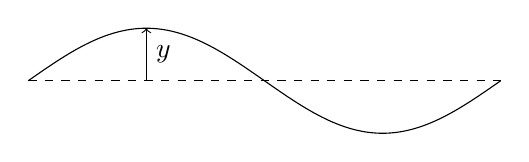
\begin{tikzpicture}
    \draw (0, 0) sin (1.5, 0.667) cos (3, 0) sin (4.5, -0.667) cos (6, 0);
    \draw [dashed] (0, 0) -- (6, 0);
    \draw [->] (1.5, 0) -- (1.5, 0.667) node [pos = 0.5, right] {$y$};
  \end{tikzpicture}
\end{center}
Suppose that $\rho(x)$ is the mass per unit length of a string. Then the restoring force on the string $\displaystyle ma = \rho \frac{\partial ^2 y}{\partial t^2}$ is proportional to the second derivative $\displaystyle\frac{\partial^2 y}{\partial x^2}$. So we obtain this wave equation.

(Why the second spatial derivative? The restoring force cannot depend on $y$ itself (translating the whole string causes no force) or on $\partial y/\partial x$ (a uniform slope has balanced forces). Only \emph{curvature}, measured by $\partial^2 y/\partial x^2$, produces a net restoring force.)

\subsubsection*{General solution (d'Alembert)}
Assuming $c$ is constant, we can factor the wave operator:
\begin{align*}
  \frac{\partial ^2 y}{\partial t^2} - c^2 \frac{\partial^2 y}{\partial x^2} &= 0\\
  \left(\frac{\partial}{\partial t} + c\frac{\partial}{\partial x}\right)\left(\frac{\partial}{\partial t} - c\frac{\partial}{\partial x}\right) y &= 0
\end{align*}
If $y = f(x + ct)$, then $(\partial_t - c\partial_x)y = 0$, so the product of operators gives zero. Similarly, $y = g(x - ct)$ satisfies $(\partial_t + c\partial_x)y = 0$. Since the equation is linear, the general solution is
\[
  y = f(x + ct) + g(x - ct),
\]
where $f$ and $g$ are arbitrary functions. This is \emph{d'Alembert's solution}: it represents a superposition of a wave travelling left (with speed $c$) and a wave travelling right (with speed $c$).

To verify this is the most general solution, substitute $\xi = x + ct$ and $\eta = x - ct$. The chain rule gives $y_{tt} - c^2 y_{xx} = -4c^2 y_{\xi\eta}$. Thus the wave equation becomes $y_{\xi\eta} = 0$, which integrates to $y = f(\xi) + g(\eta)$.

How many boundary conditions do we need to have a unique solution? In ODEs, we simply count the order of the equation. In PDEs, we have to count over all variables. In this case, we need 2 boundary conditions and 2 initial conditions. For example, we can have:
\begin{itemize}
  \item Initial conditions: at $t = 0$,
    \begin{gather*}
      y = \frac{1}{1 + x^2}\\
      \frac{\partial y}{\partial t} = 0
    \end{gather*}
  \item Boundary conditions: $y \to 0$ as $x \to \pm \infty$.
\end{itemize}
We know that the solution has the form
\[
  y = f(x + ct) + g(x - ct).
\]
The first initial condition give
\[
  f(x) + g(x) = \frac{1}{1 + x^2}\tag{1}
\]
The second initial condition gives
\[
  \frac{\partial y}{\partial t} = cf'(x) - cg'(x)\tag{2} = 0
\]
From (2), we know that $f' = g'$. So $f$ and $g$ differ by a constant. wlog, we can assume that they are indeed equal, since if we had, say, $f = g + 2$, then we can let $y = (f(x + ct) + 1) + (g(x - ct) + 1)$ instead, and the new $f$ and $g$ are equal.

From (1), we must have
\[
  f(x) = g(x) = \frac{1}{2(1 + x^2)}
\]
So, overall,
\[
  y = \frac{1}{2}\left[\frac{1}{1 + (x + ct)^2} + \frac{1}{1 + (x - ct)^2}\right]
\]
Where we substituted $x$ for $x +ct$ and $x - ct$ in $f$ and $g$ respectively.

\subsection{The diffusion equation}
The \emph{diffusion equation} (or \emph{heat equation}) models heat conduction in a solid:
\[
  \frac{\partial T}{\partial t} = \kappa \frac{\partial^2 T}{\partial x^2},
\]
where $T(x, t)$ is the temperature and $\kappa > 0$ is the \emph{thermal diffusivity}. This is classified as a \emph{parabolic PDE}.

Unlike the wave equation (where acceleration $\propto$ curvature), here the rate of change $\partial T/\partial t$ is directly proportional to curvature $\partial^2 T/\partial x^2$. This makes the diffusion equation \emph{dissipative}: irregularities smooth out over time rather than propagating as waves.

\begin{eg}[Semi-infinite heated bar]
  Consider a semi-infinite bar ($x \geq 0$) that is initially at temperature zero, then heated at the end $x = 0$ for $t > 0$:

  Suppose $T(x,0) = 0$, $T(0, t) = H(t) =
  \begin{cases}
    0 & t < 0\\
    1 & t > 0
  \end{cases}$, and $T(x, t)\to 0$ as $x\to \infty$. In words, the bar is initially cold, then suddenly heated at one end.

  We seek a \emph{similarity solution}---a solution where $T$ depends on $x$ and $t$ only through a particular combination. The natural length scale for diffusion over time $t$ is $\sqrt{\kappa t}$, suggesting we try $T(x, t) = \theta(\eta)$ where
  \[
    \eta = \frac{x}{2\sqrt{\kappa t}}
  \]
  is the \emph{similarity variable}.

  Applying the chain rule, we have
  \begin{align*}
    \frac{\partial T}{\partial x} &= \frac{\d \theta}{\d \eta} \frac{\partial \eta}{\partial x}\\
    &= \frac{1}{2\sqrt{\kappa t}} \theta'(\eta)\\
    \frac{\partial^2 T}{\partial x^2} &= \frac{1}{2\sqrt{\kappa t}} \frac{\d\theta'}{\d\eta}\frac{\partial \eta}{\partial x}\\
    &= \frac{1}{4\kappa t}\theta''(\eta)\\
    \frac{\partial T}{\partial t} &= \frac{\d \theta}{\d \eta}\frac{\partial \eta}{\partial t}\\
    &= -\frac{1}{2}\frac{x}{2\sqrt{\kappa}}\frac{1}{t^{3/2}} \theta'(\eta)\\
    &= -\frac{\eta}{2t}\theta'(\eta)
  \end{align*}
  Putting this into the diffusion equation yields
  \begin{align*}
    -\frac{\eta}{2t}\theta' &= \kappa \frac{1}{4\kappa t}\theta''\\
    \theta'' + 2\eta\theta' &= 0
  \end{align*}
  This is an ordinary differential equation for $\theta(\eta)$. This can be seen as a first-order equation for $\theta'$ with non-constant coefficients. Use the integrating factor $\mu = \exp(\int 2\eta \;\d \eta) = e^{\eta^2}$. So
  \begin{align*}
    (e^{\eta^2}\theta')' &= 0\\
    \theta' &= Ae^{-\eta^2}\\
    \theta &= A\int_0^\eta e^{-u^2}\;\d u + B\\
    &= \alpha\erf(\eta) + B
  \end{align*}
  where $\erf(\eta) = \frac{2}{\sqrt{\pi}} \int_0^\eta e^{-u^2}\;\d u$ from statistics, and $\erf(\eta)\to 1$ as $\eta\to \infty$.

  Now look at the boundary and initial conditions, (recall $\eta = x/(2\sqrt{\kappa t})$) and express them in terms of $\eta$. As $x \to 0$, we have $\eta \to 0$. So $\theta = 1$ at $\eta = 0$.

  Also, if $x\to \infty, t\to 0^+$, then $\eta \to \infty$. So $\theta \to 0$ as $\eta \to \infty$.

  From $\theta(0) = 1$, we get $B = 1$. From $\theta \to 0$ as $\eta \to \infty$, we need $\alpha = -1$. Thus $\theta = 1 - \erf(\eta) = \erfc(\eta)$, the \emph{complementary error function}. The solution is
  \[
    T = \erfc\left(\frac{x}{2\sqrt{\kappa t}}\right).
  \]
  At any fixed time $t$, the temperature profile looks like:
  \begin{center}
    \begin{tikzpicture}[xscale=3]
      \draw [->] (0, 0) -- (2.1, 0) node [right] {$x$};
      \draw [->] (0, 0) -- (0, 3) node [above] {$T$};

      %% approximation of error function
      \draw [mblue, semithick, domain=0:2] plot (\x, {2.5 * (1 + 0.278393 * \x + 0.230389*\x*\x + 0.000972*\x*\x*\x + 0.078108 * \x*\x*\x*\x)^(-4)});
    \end{tikzpicture}
  \end{center}
  The heat penetrates a distance of order $\sqrt{\kappa t}$, which grows with time. For a finite bar of length $L$, we can treat it as semi-infinite provided $\sqrt{\kappa t} \ll L$, i.e., $t \ll L^2/\kappa$.
\end{eg}
\end{document}
